\section{Background Estimation}

\subsection{Irreducible Backgrounds}
\label{sec:irrbkgd}
\subsubsection{\qqZZ~ Modelling}
\label{sec:redbkgd}

The \qqZZ~ background is generated at NLO, while the fully differential cross section has been computed at 
NNLO~\cite{Grazzini2015407}, but are not yet available in a partonic level event generator. Therefore NNLO/NLO 
$k$-factors for the \qqZZ~background process are applied to the {\sc powheg} sample. The inclusive cross 
sections obtained using the same PDF and renormalization and factorization scales as the {\sc powheg} sample
at LO, NLO, and NNLO are shown in Table~\ref{tab:qqZZXS}. The NNLO/NLO $k$-factors are applied in the analysis
differentally as a function of $m(\cPZ\cPZ)$. 

Additional NLO electroweak corrections which depend on the initial state quark flavor and kinematics
are also applied to the \qqZZ~ background process in the region $m(\cPZ \cPZ)>2m(\cPZ)$ where the 
corrections have been computed. The differential QCD and electroweak $k$-factors can be seen in 
Figure~\ref{fig:qqZZKfactor}.

\begin{table}[h]
    \centering
    \begin{tabular}{|l|c|c|} 
\hline %----------------------------------------------------------------
QCD Order  & $\sigma_{2\ell2\ell^{\prime}} (\mathrm{fb})$  & $\sigma_{4\ell} (\mathrm{fb})$  \\
\hline %----------------------------------------------------------------
LO    & 218.5$^{+16\%}_{-15\%}$ & 98.4$^{+13\%}_{-13\%}$ \\
NLO   & 290.7$^{+5\%}_{-8\%}$   & 129.5$^{+4\%}_{-6\%}$ \\
NNLO  & 324.0$^{+2\%}_{-3\%}$   & 141.2$^{+2\%}_{-2\%}$ \\
\hline %----------------------------------------------------------------
    \end{tabular}
    \caption{Cross sections for \qqZZ~ production at 13 \TeV}
    \label{tab:qqZZXS}
\end{table}

%=======
\begin{figure}[!htb]
\vspace*{0.3cm}
\begin{center}
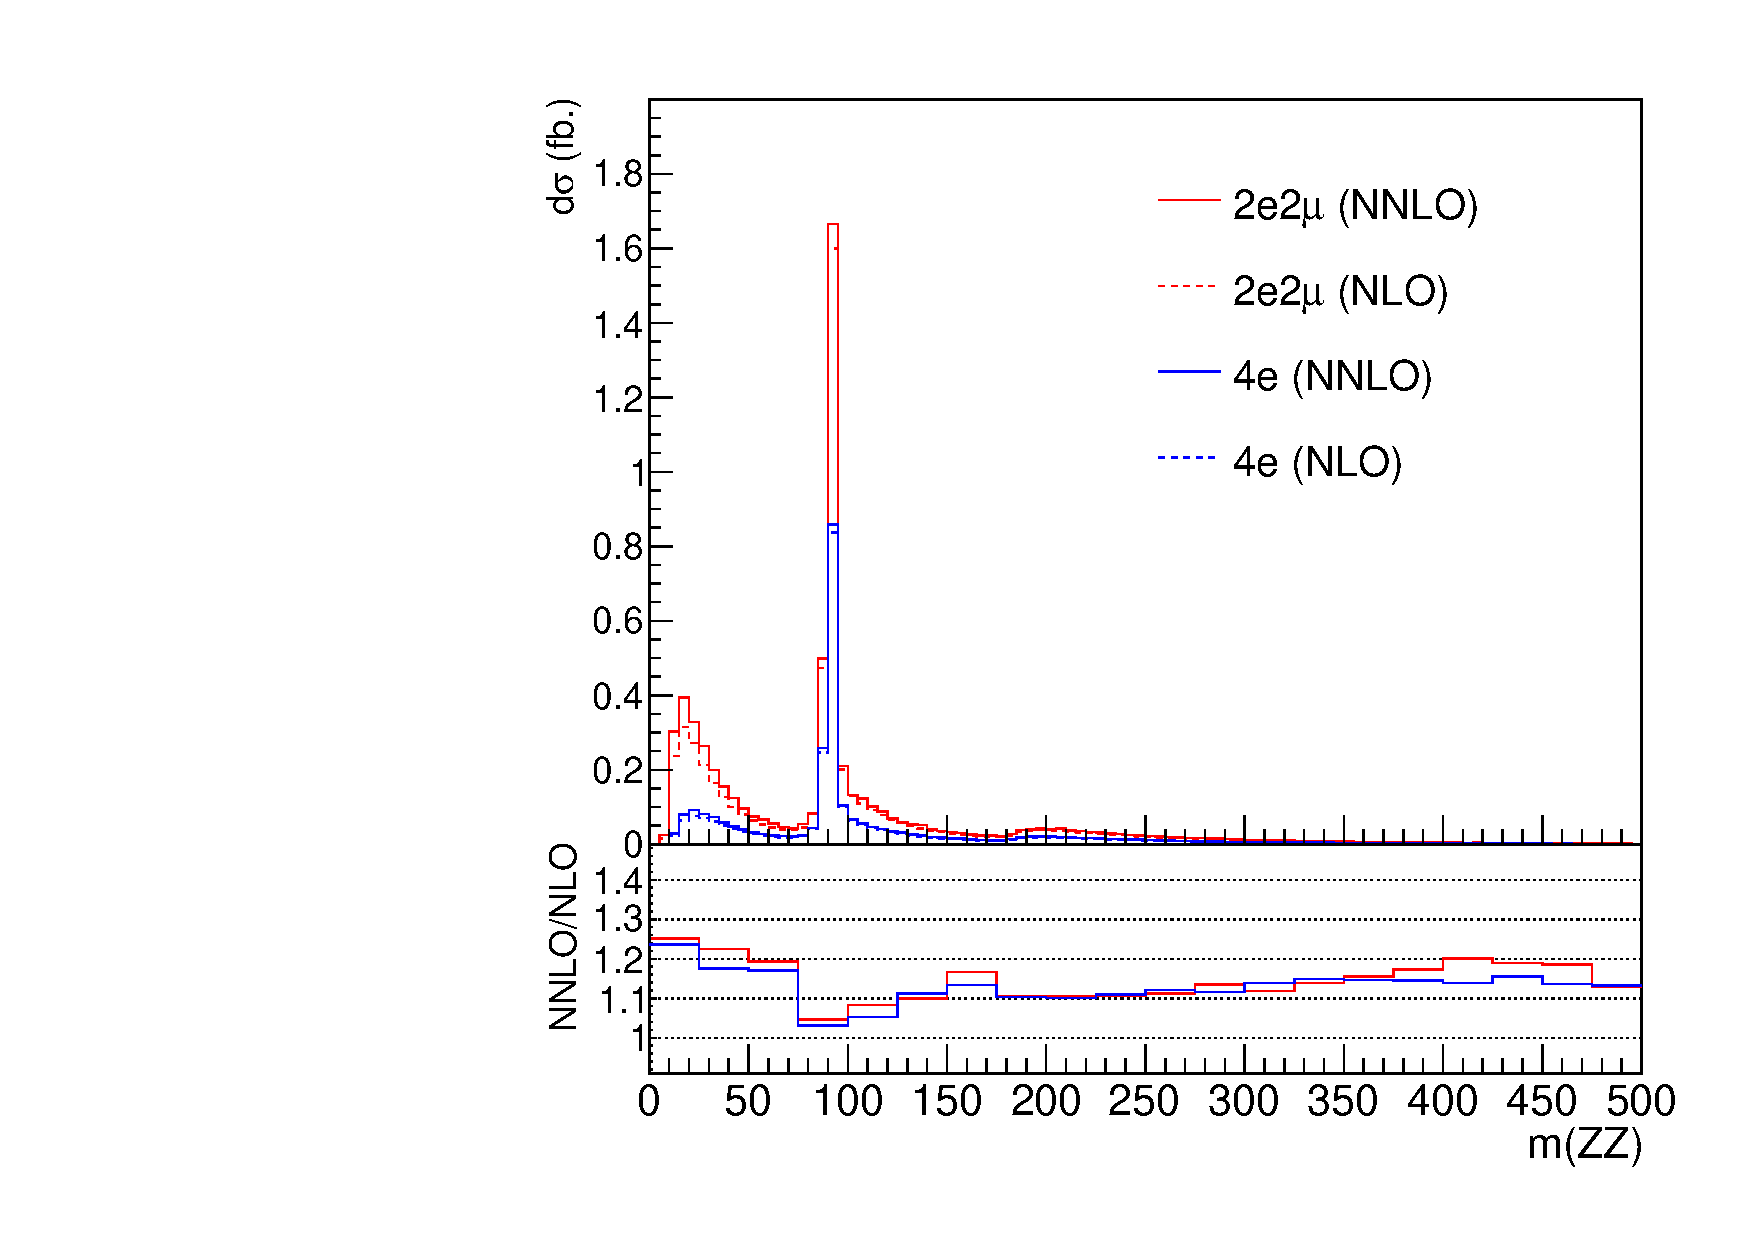
\includegraphics[width=0.48\textwidth]{Figures/IrrBkg/Kfactor_qqZZ_mZZ.pdf}
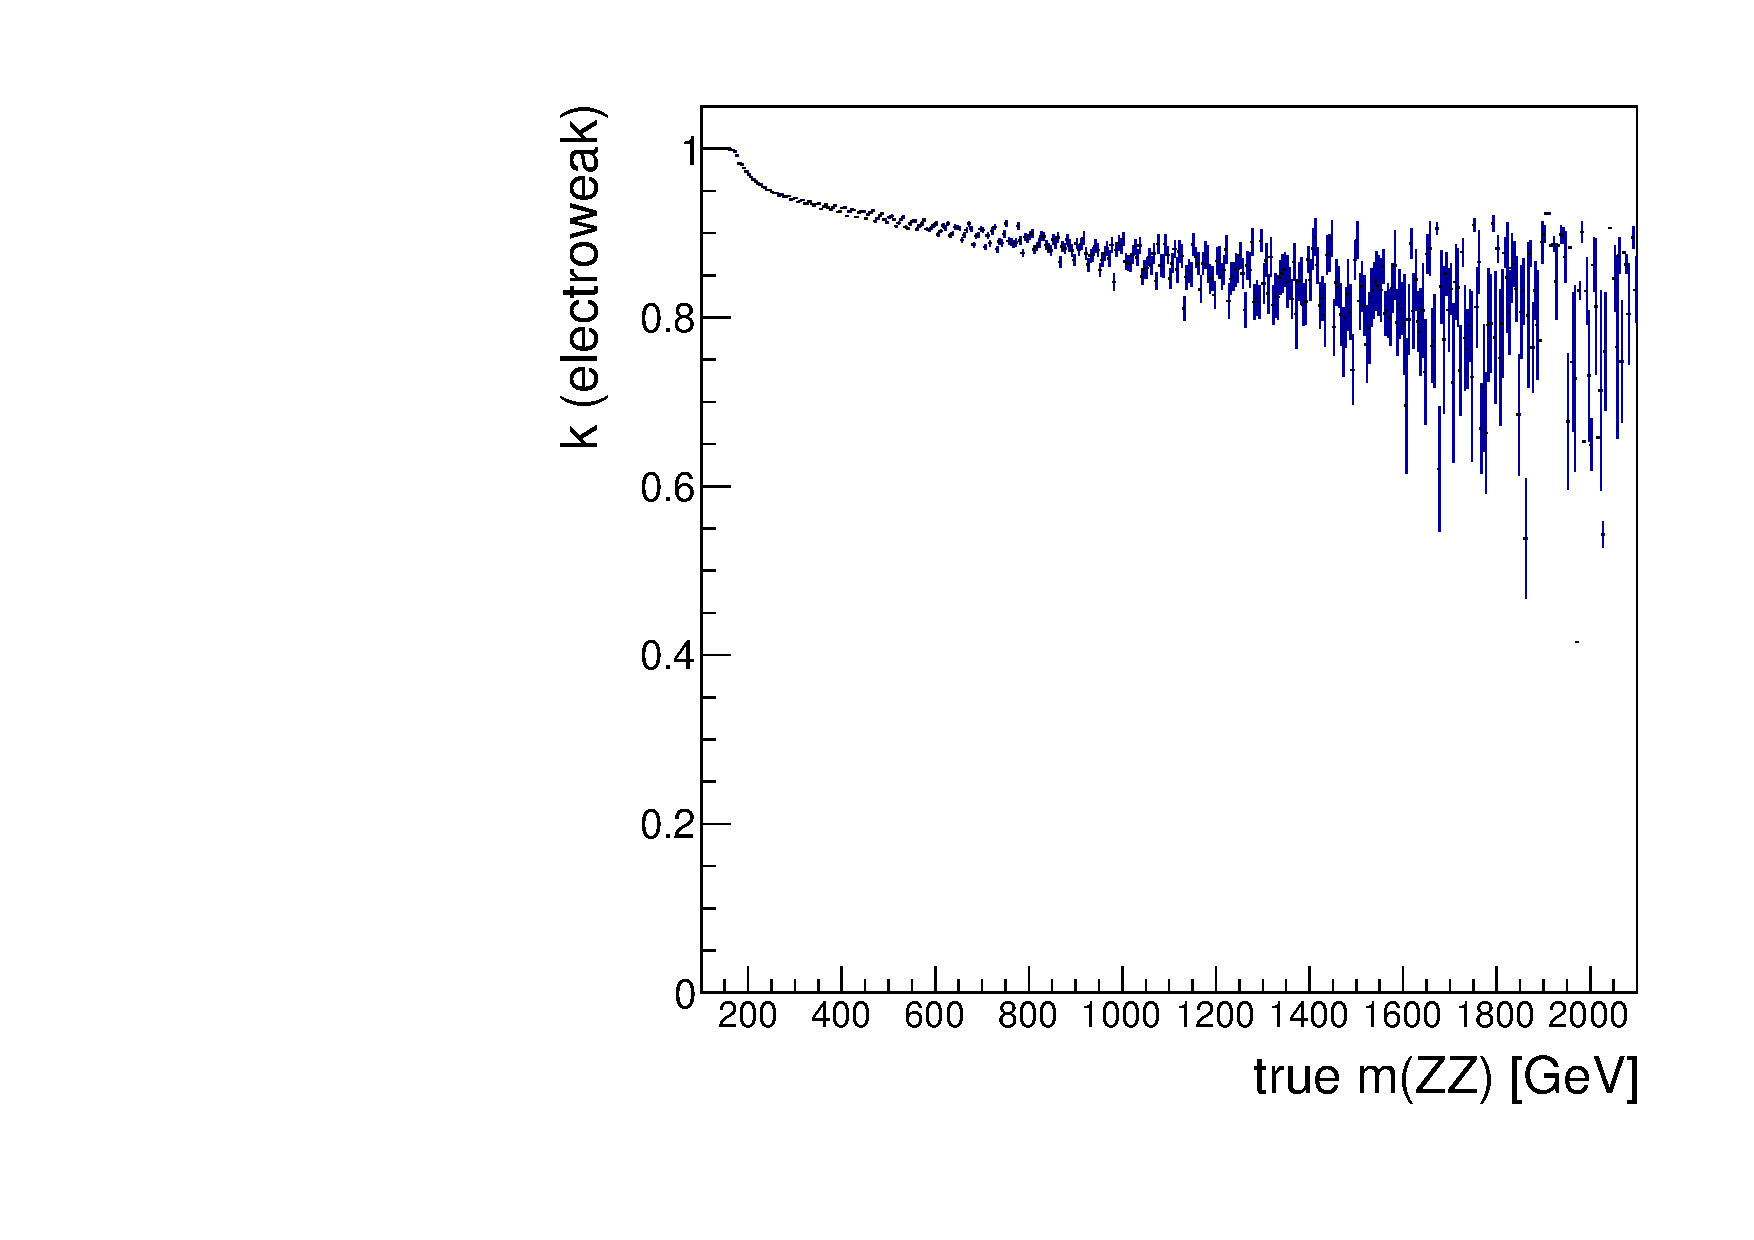
\includegraphics[width=0.48\textwidth]{Figures/IrrBkg/K_ewk_qqZZ.pdf} 
\caption{Left: NNLO/NLO QCD K factor for the \qqZZ~ background as a function of $m(ZZ)$ for the $4\ell$ and $2\ell2\ell^{\prime}$ final states. Right: NLO/NLO electroweak K factor for the \qqZZ~ background as a function of $m(ZZ)$.
\label{fig:qqZZKfactor}}
\end{center}
\end{figure}


\subsubsection{\ggZZ~ Modelling}

Event simulation for the $\ggZZ$ background is done at LO with the generator \MCFM~7.0~\cite{MCFM,Campbell:2011bn,Campbell:2013una}.
Although no exact calculation exists beyond the LO for the $\ggZZ$ background, 
it has been recently shown~\cite{Bonvini:1304.3053} 
that the soft collinear approximation is able to describe the background cross section and the 
interference term at NNLO\@. Further calculations also show that the K factors are very similar at NLO for the signal 
and background~\cite{Melnikov:2015laa} and at NNLO for the signal and interference terms~\cite{Li:2015jva}. Therefore, the same K factor 
is used for the signal and background~\cite{Passarino:1312.2397v1}. The NNLO K factor for the signal is obtained as a function of $\mllll$ 
using the \textsc{hnnlo}~v2 Monte Carlo program~\cite{Catani:2007vq,Grazzini:2008tf,Grazzini:2013mca} by calculating the NNLO and LO 
$\Pg\Pg\to\PH\to2\ell2\ell^\prime$ cross sections at the small $\PH$ boson decay width of $4.07$~\MeV and taking their ratios. The NNLO as 
well as the NLO K factors and the cross sections from which they are derived are illustrated in Figure~\ref{fig:ggHZZXsecKfactor}, 
along with the NNLO, NLO and LO cross sections at the SM $\PH$ boson decay width~\cite{Heinemeyer:2013tqa}.
 
\begin{figure}[!htb]
\centering
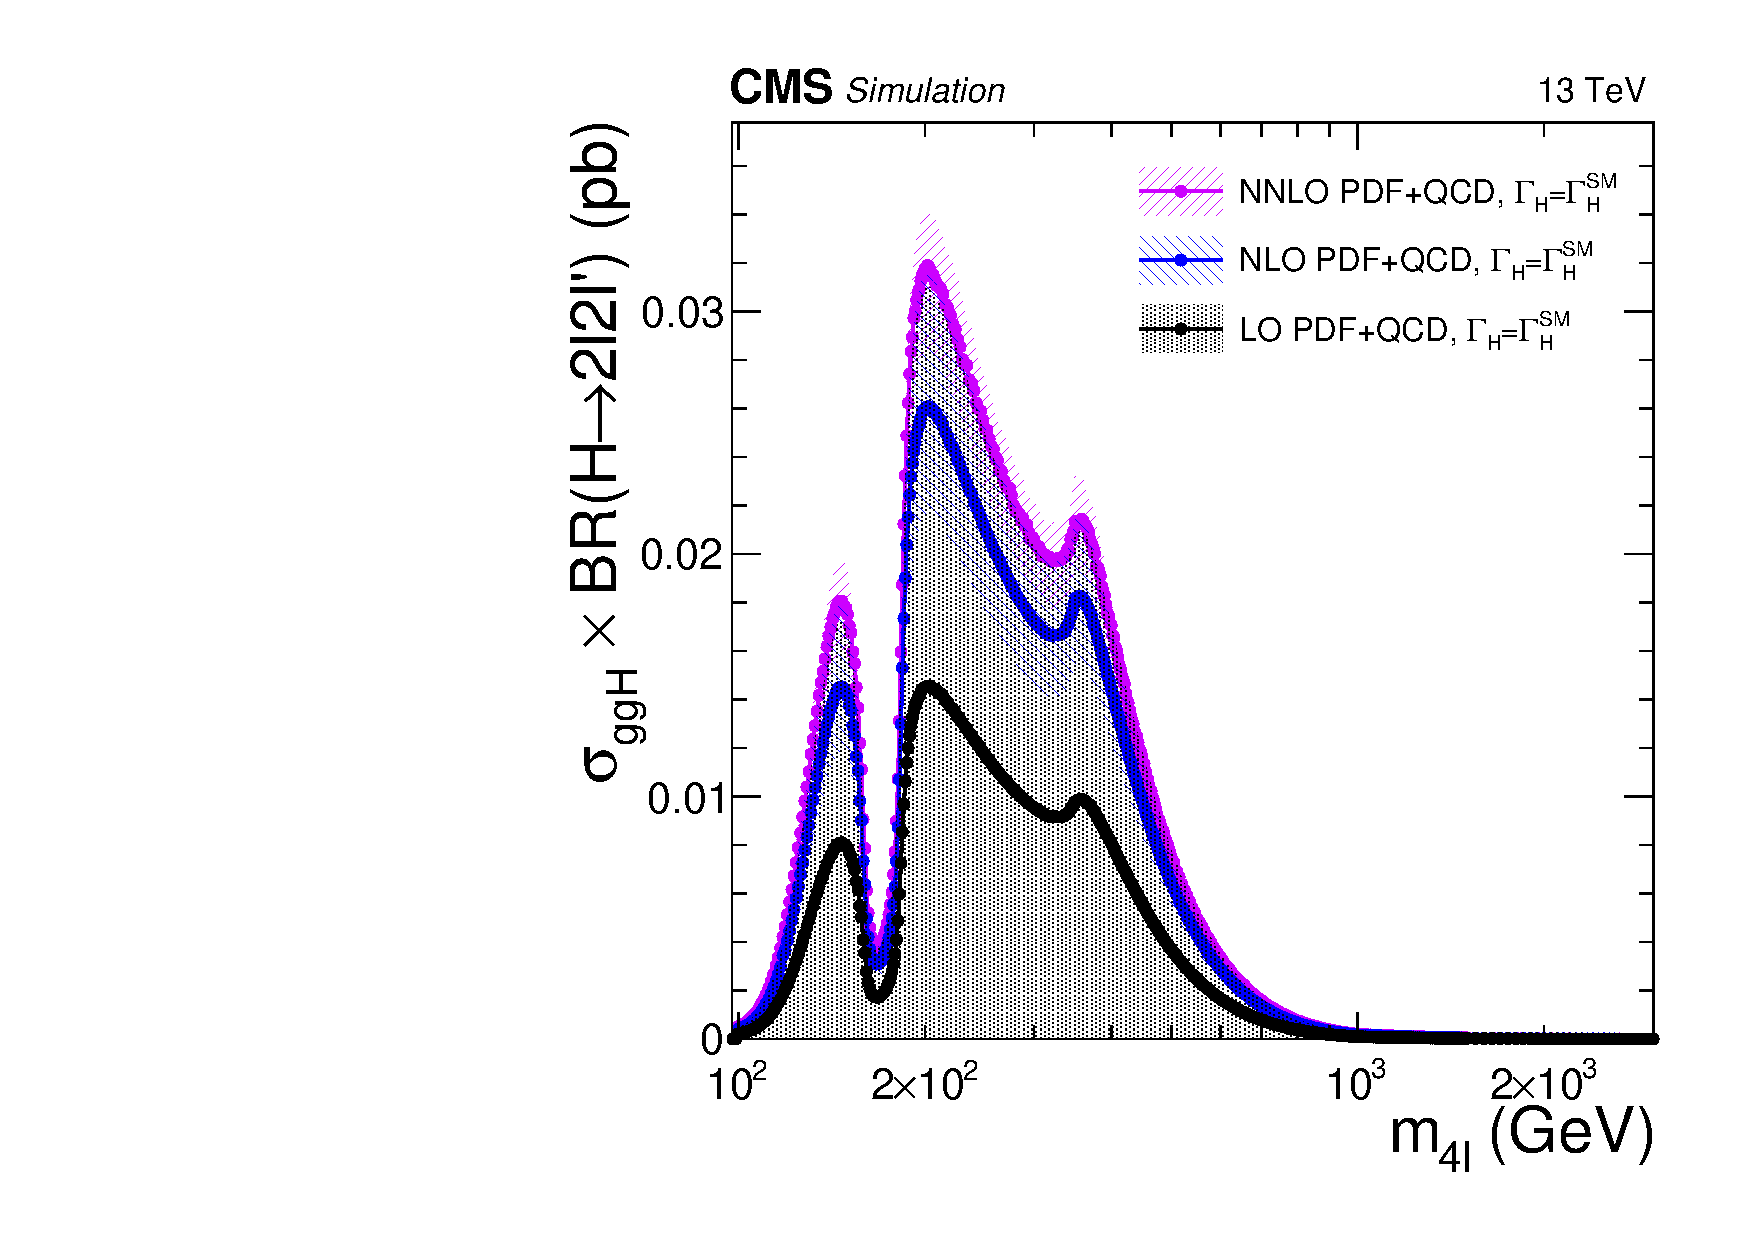
\includegraphics[width=0.48\linewidth]{Figures/IrrBkg/cCompare_hnnlo_ggHZZ2l2l_xsec.pdf}
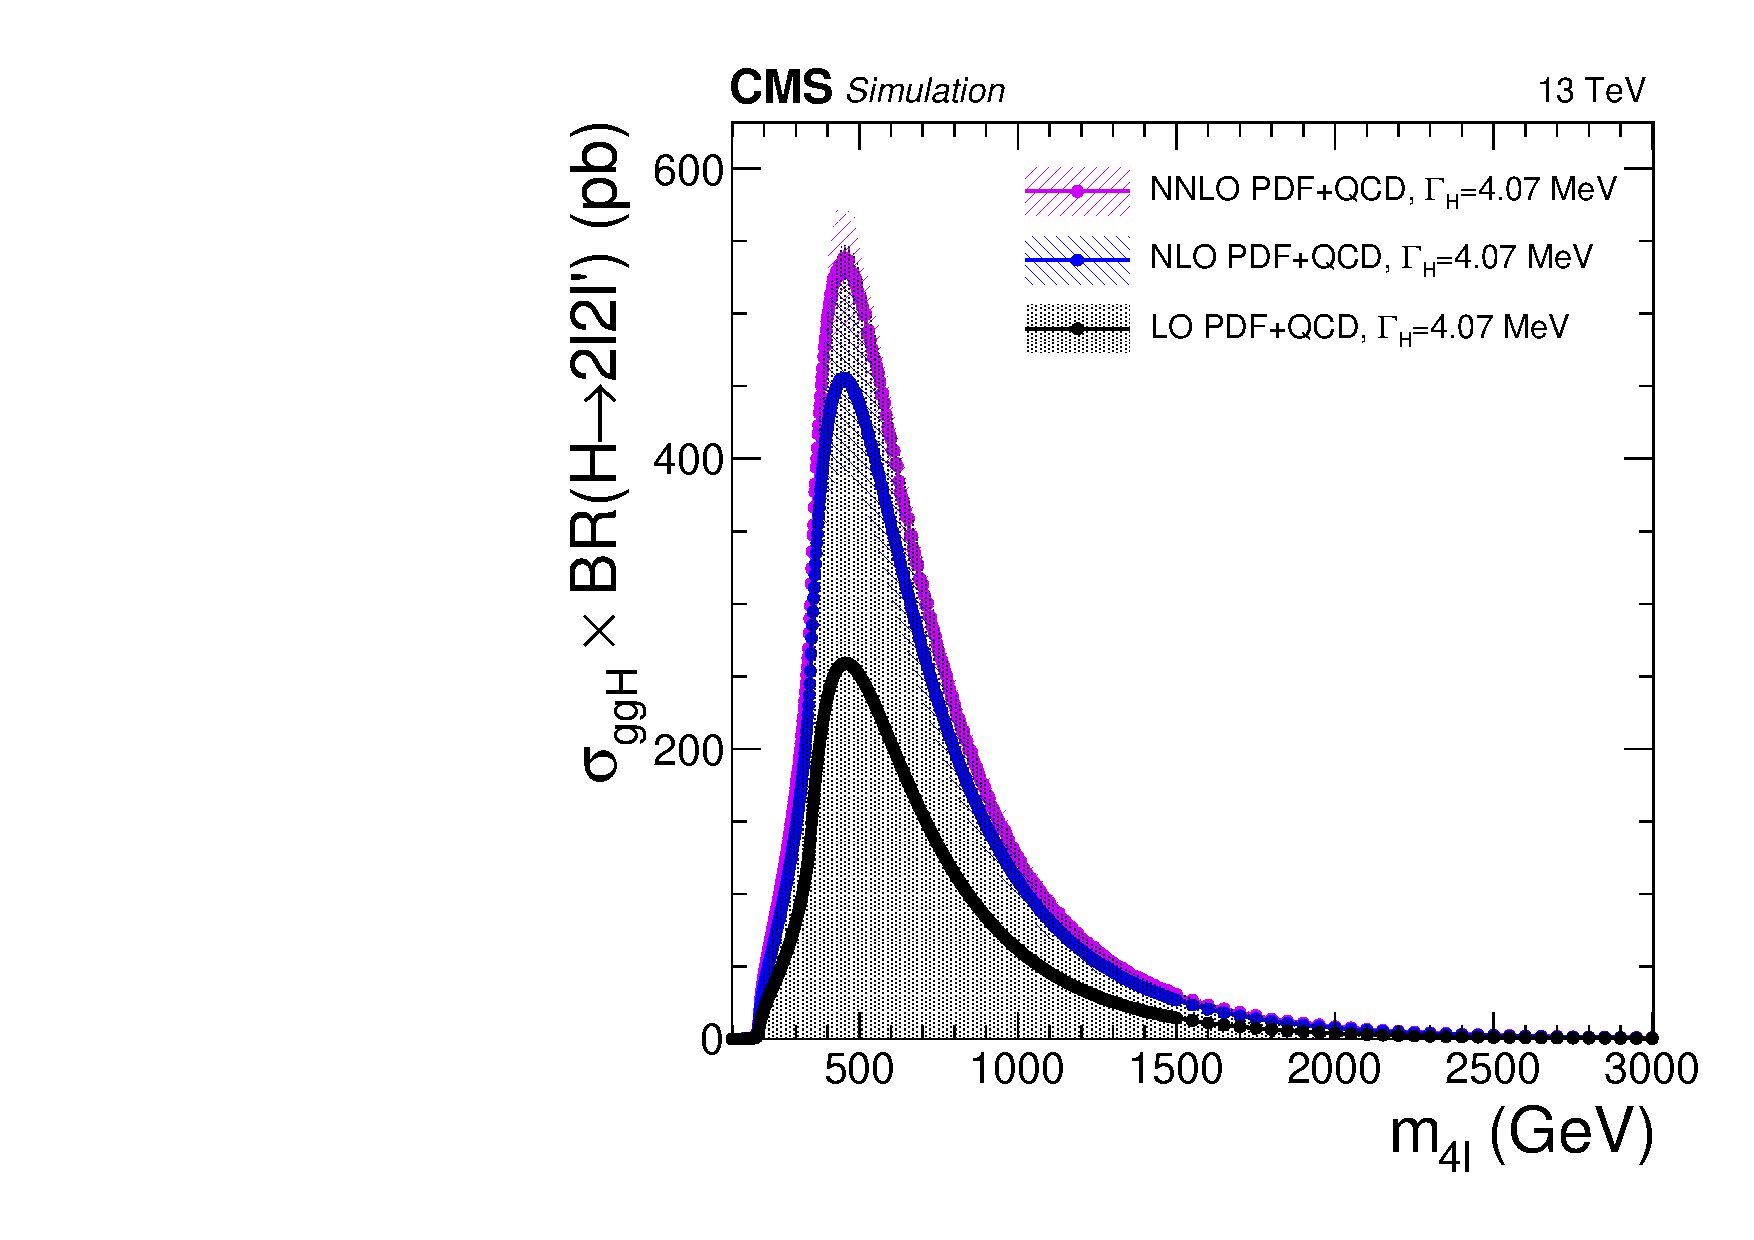
\includegraphics[width=0.48\linewidth]{Figures/IrrBkg/cCompare_hnnlo_ggHZZ2l2l_narrowwidth_xsec.pdf}\\
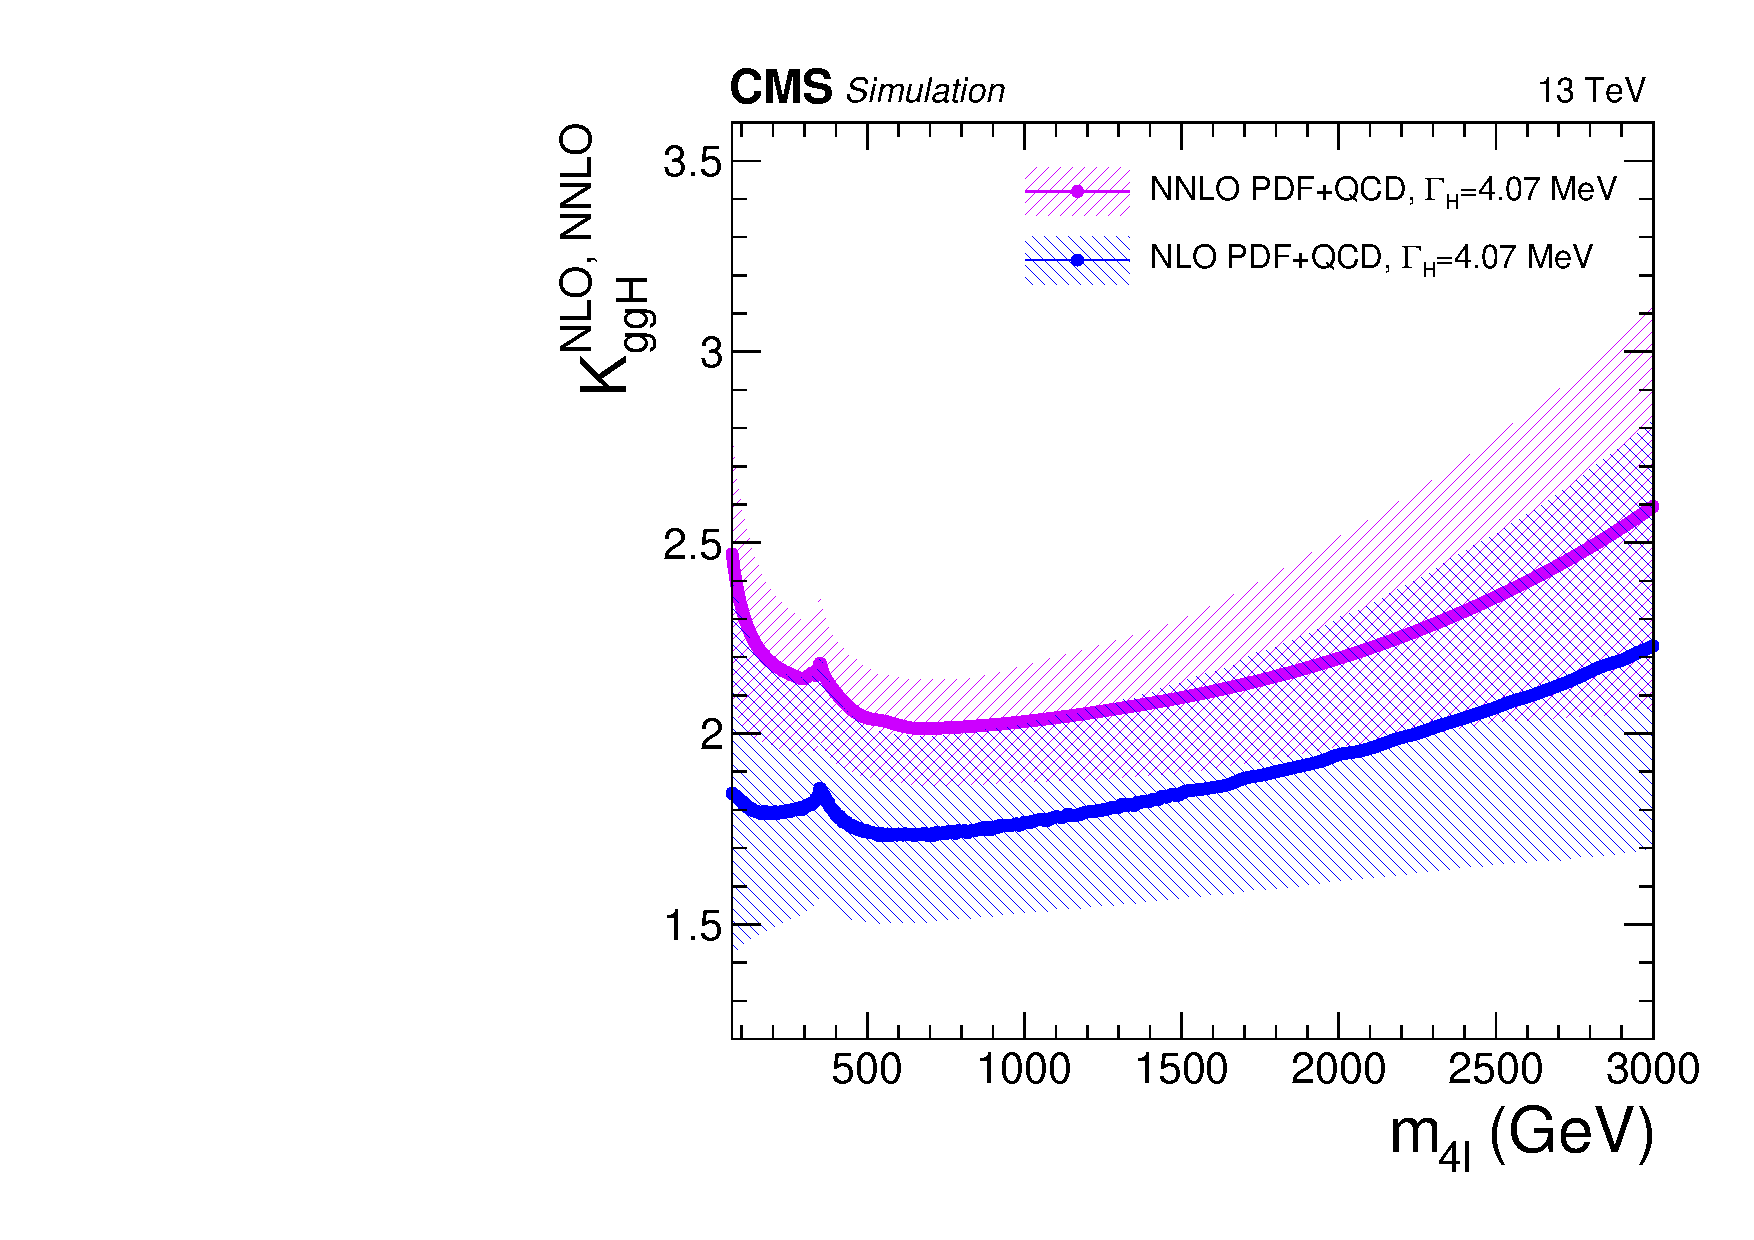
\includegraphics[width=0.48\linewidth]{Figures/IrrBkg/cCompare_hnnlo_ggHZZ2l2l_narrowwidth_kfactor.pdf}
\caption{$\Pg\Pg\to\PH\to2\ell2\ell^\prime$ cross sections at NNLO, NLO and LO at each $\PH$ boson pole mass using the SM $\PH$ boson decay width  (top left) or at the fixed and small decay width of $4.07$~MeV (top right). The cross sections using the fixed value are used to obtain the K factor for both the signal and the continuum background contributions as a function of $\mllll$ (bottom).
}
\label{fig:ggHZZXsecKfactor}
\end{figure}



\clearpage

\subsection{Reducible Background}
%\textbf{work on-going to improve the Z+X estimation and reduce its uncertainty}
\label{sec:zxIntr}
The reducible background for the $H\to ZZ\to 4\ell $ analysis, hereafter called $Z+X$, originates from processes which contain one or more nonprompt leptons in the four lepton final state. 
The main sources of nonprompt leptons are non-isolated electrons and muons coming from decays of heavy flavour mesons, misreconstructed jets (usually originating from light flavour quarks) and electrons from $\gamma$ conversions. 
In this discussion, we will consider a ``fake lepton'' any jet misreconstructed as a lepton and any lepton originating from a heavy meson decay.
Similarly, any electron originating from a photon conversion will be considered a ``fake electron''.

In the $H\to ZZ\to 4\ell $ analysis, the rate of these background processes is estimated by measuring the $f_{e}$ and $f_{\mu}$ probabilities for fake electrons and fake muons which do pass the {\bf loose} selection criteria (defined in Section~\ref{sec:eleReco} and~\ref{sec:muonReco}) to also pass the final selection criteria (defined in Section~\ref{sec:zzcandsel}).  
These probabilities, hereafter referred to as fake ratios or fake rates (FR), are applied in dedicated control samples in order to extract the expected background yield in the signal region. 

In the following section, two independent methods are presented to measure both the yields and shapes of the reducible background, called Opposite-Sign (OS) method and Same-Sign (SS) method. The final result combines the outcome of the two approaches. The methods are the same as in the 2016 analysis, although additional cross checks have been performed. 


% OS method

\subsubsection{Reducible Background Estimate with Opposite-Sign Leptons}
\label{sec:zxOS}
\paragraph{Fake Rate Determination (OS method)}
In order to measure the lepton fake ratios $f_{e}$ and $f_{\mu}$, we select samples of $Z(\ell\ell)+e$ and $Z(\ell\ell)+\mu$ events that are expected to be completely dominated by final states which include a $Z$ boson and a fake lepton. 
These events are required to have two same flavour, opposite charge leptons with $p_{T} > 20/10$~GeV passing the tight selection criteria, thus forming the $Z$ candidate. In addition, there is exactly one lepton passing the loose selection criteria as defined above. 
This lepton is used as the probe lepton for the fake ratio measurement. The invariant mass of this lepton and the opposite sign lepton from the reconstructed $Z$ candidate should satisfy $m_{2l} > 4$~GeV. 


The fake ratios are evaluated using the tight requirement 
$|M_{inv}(\ell_{1},\ell_{2}) - M_{Z}| < 7 $~GeV, to reduce the 
contribution from photon (asymmetric) conversions populating low masses. 
The fake ratios are measured in bins of the transverse momentum of the loose lepton in the barrel and endcap regions. 
The electron and muon fake rates are measured within 
$|M_{inv}(\ell_{1},\ell_{2}) - M_{Z}| < 7 $~GeV and $E_{\mathrm{T}}^\text{miss}  < $ 25~GeV, 
separately for the 2016, 2017 and 2018 data, and are shown in Figure~\ref{fig:os_fakerates}. 


\paragraph{Fake Rate Application (OS method)}
\label{sec:zxA}

Two control samples are obtained as subsets of the four lepton events
which pass the first step of the selection ({\it First Z} step, see
section~\ref{sec:zzcandsel}), requiring an additional pair of identified
loose leptons of same flavour 
and opposite charge, that pass the ${\rm SIP_{3D}}$, dxy and dz cuts. 
The events must satisfy all kinematic cuts applied for the {\it Higgs phase space} selection
(see~\ref{sec:zzcandsel}).

The first control sample is obtained by
requiring that the two loose leptons, which do not make the $Z_1$ candidate, 
do not pass the final selection criteria, while the other two leptons pass
the final selection criteria by definition of the $Z_1$. 
This sample is denoted as ``2 Prompt + 2 Fail'' ({\it 2P+2F}) sample. 
It is expected to be populated with events that intrinsically have only two prompt leptons 
(mostly $DY$, with a small fraction of $t \bar{t}$ and $Z \gamma$ events).
The second control sample is obtained by requiring one of
the four leptons not to pass the final identification criteria 
and selection cuts on SIP, dxy and dz and is denoted as ``3 Prompt + 1 Fail'' ({\it 3P+1F}) sample. 
%======= 
\begin{figure}[!]
\begin{center}
    {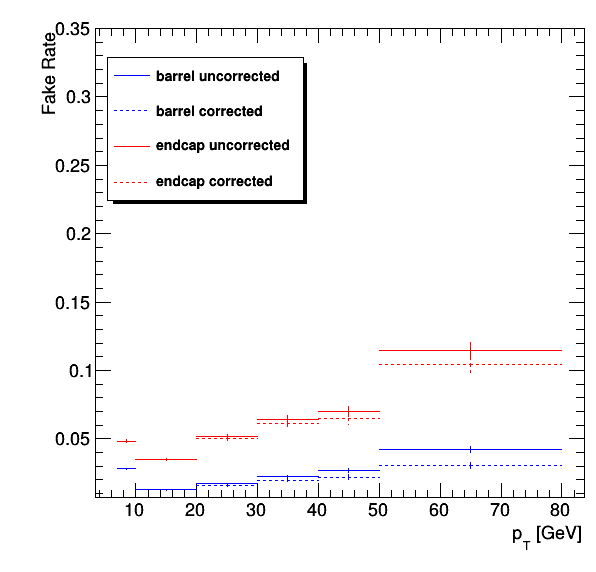
\includegraphics [width=0.45\textwidth] {Figures/RedBkg/FR/FR_OS_electrons_2016.png}}
    {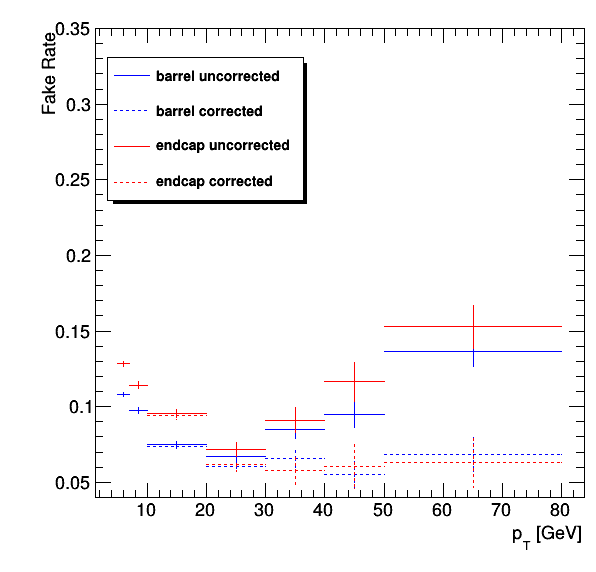
\includegraphics [width=0.45\textwidth] {Figures/RedBkg/FR/FR_OS_muons_2016.png}} \\
    {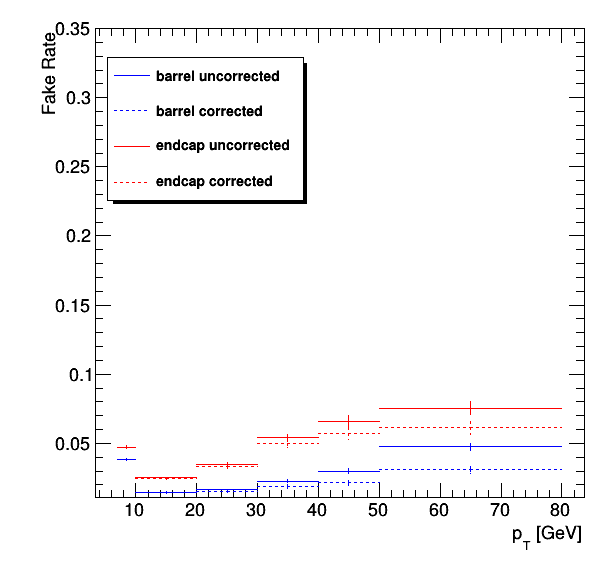
\includegraphics [width=0.45\textwidth] {Figures/RedBkg/FR/FR_OS_electrons_2017.png}}
    {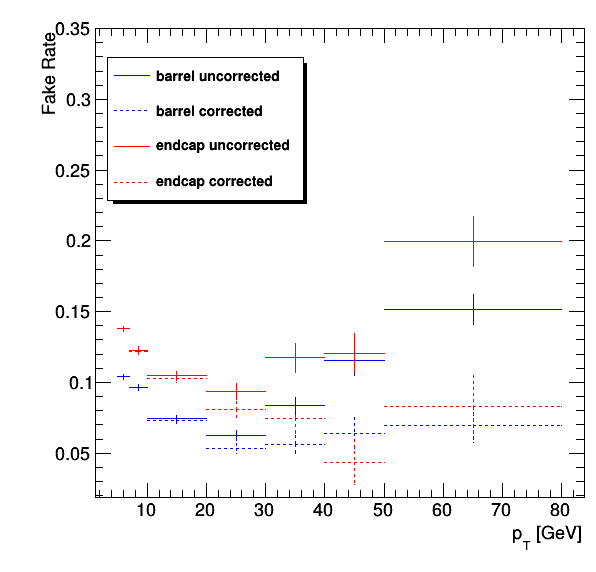
\includegraphics [width=0.45\textwidth] {Figures/RedBkg/FR/FR_OS_muons_2017.png}} \\
    {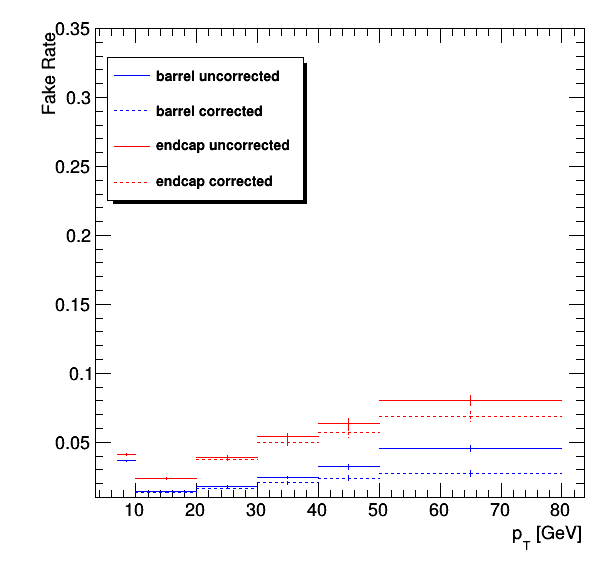
\includegraphics [width=0.45\textwidth] {Figures/RedBkg/FR/FR_OS_electrons_2018.png}}
    {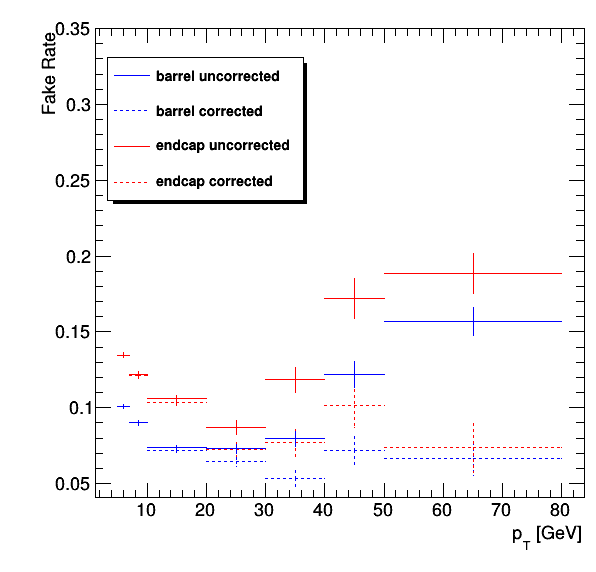
\includegraphics [width=0.45\textwidth] {Figures/RedBkg/FR/FR_OS_muons_2018.png}} 
\caption{
Fake rates as a function of the probe $p_T$ for  electrons (left) and muons (right) which satisfy the loose selection criteria, measured in
a $Z(\ell\ell)+\ell$ sample in the 2016 (top), 2017 (middle) and 2018 (bottom) data at $13$~TeV.
The barrel selection includes electrons (muons) up to $|\eta|$ = 1.479 (1.2). The fake rates are shown before (dotted lines) and after (plain line) removal of WZ contribution from MC.
}
\label{fig:os_fakerates}
\end{center}
\end{figure}
%=======  
The other three leptons should pass the final selection criteria. 

It is expected to be populated with the type of events that populate the
2P+2F region, albeit with different relative proportions,
as well as with $WZ$ events that intrinsically have three prompt leptons.

The control samples obtained in this way, orthogonal by construction
to the signal region, are enriched with fake leptons and are used to
estimate the reducible background in the signal region. 
The invariant mass distribution of events selected in the 2P+2F control sample
is shown in Figures~\ref{fig:2P2F_dataMC2016},~\ref{fig:2P2F_dataMC2017} and~\ref{fig:2P2F_dataMC2018}. 
\begin{figure}[!htb]
\begin{center}
        \subfigure[]{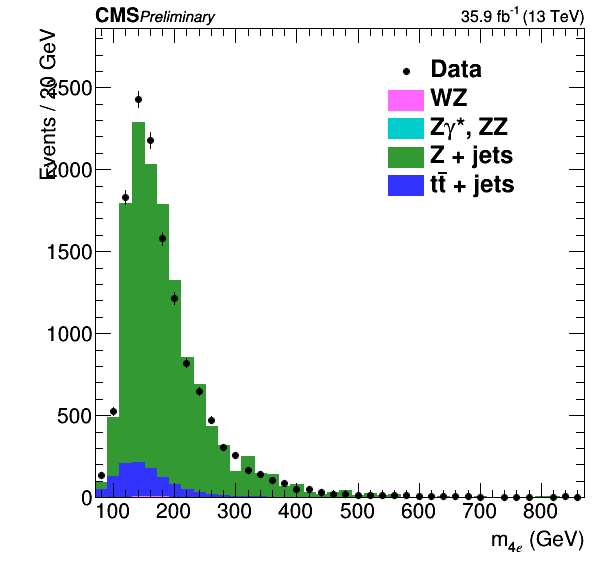
\includegraphics[width=0.45\textwidth]{Figures/RedBkg/M4l_dataMC/M4l_OS_2P2F_4e_2016_Inclusive.png}}
        \subfigure[]{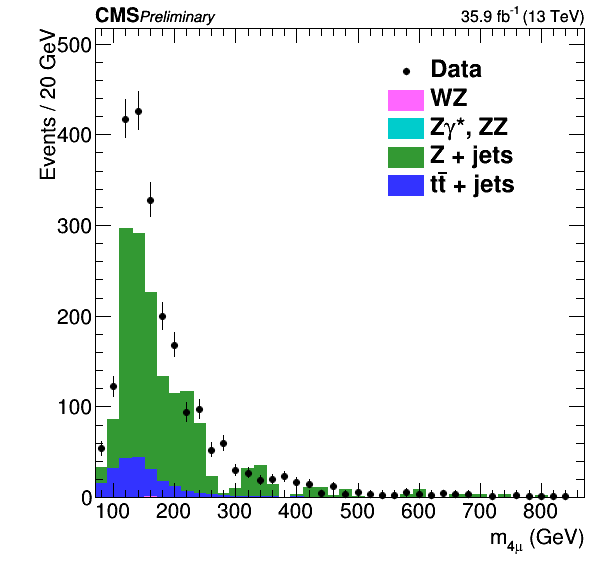
\includegraphics[width=0.45\textwidth]{Figures/RedBkg/M4l_dataMC/M4l_OS_2P2F_4mu_2016_Inclusive.png}}  \\
        \subfigure[]{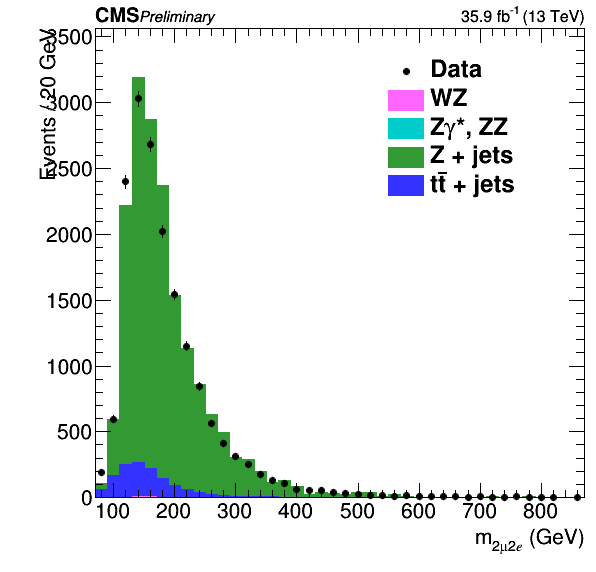
\includegraphics[width=0.45\textwidth]{Figures/RedBkg/M4l_dataMC/M4l_OS_2P2F_2mu2e_2016_Inclusive.png}}
        \subfigure[]{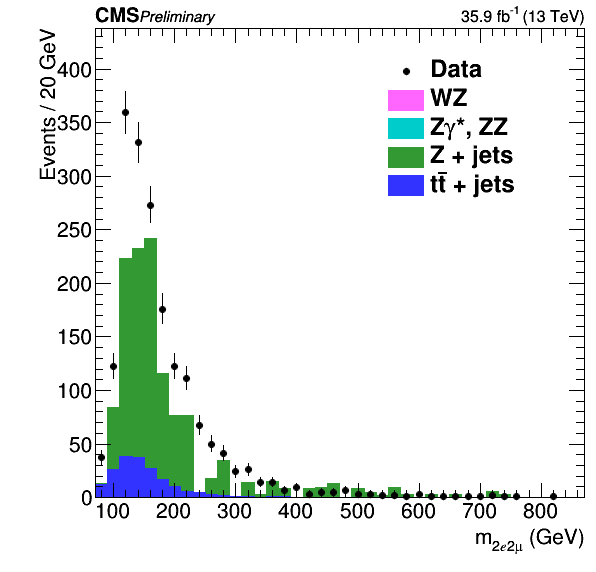
\includegraphics[width=0.45\textwidth]{Figures/RedBkg/M4l_dataMC/M4l_OS_2P2F_2e2mu_2016_Inclusive.png}} \\
\caption{
Invariant mass distribution of the events selected in the 2P+2F control sample in the
2016 dataset for all the considered channels: $4e$ (a), $4\mu$ (b), $2\mu2e$ (c) and $2e2\mu$ (d).
}
\label{fig:2P2F_dataMC2016}
\end{center}
\end{figure}

\begin{figure}[!htb]
\begin{center}
        \subfigure[]{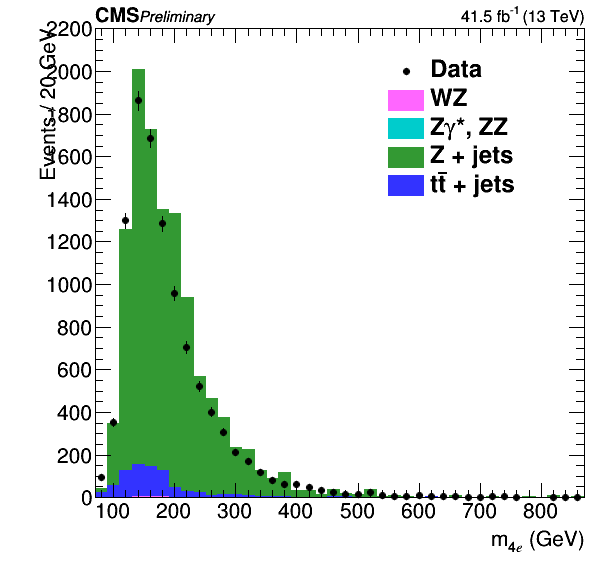
\includegraphics[width=0.45\textwidth]{Figures/RedBkg/M4l_dataMC/M4l_OS_2P2F_4e_2017_Inclusive.png}}
        \subfigure[]{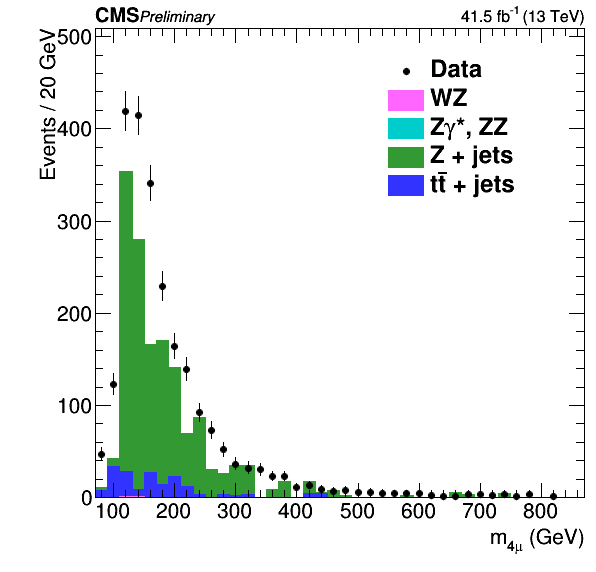
\includegraphics[width=0.45\textwidth]{Figures/RedBkg/M4l_dataMC/M4l_OS_2P2F_4mu_2017_Inclusive.png}}  \\
        \subfigure[]{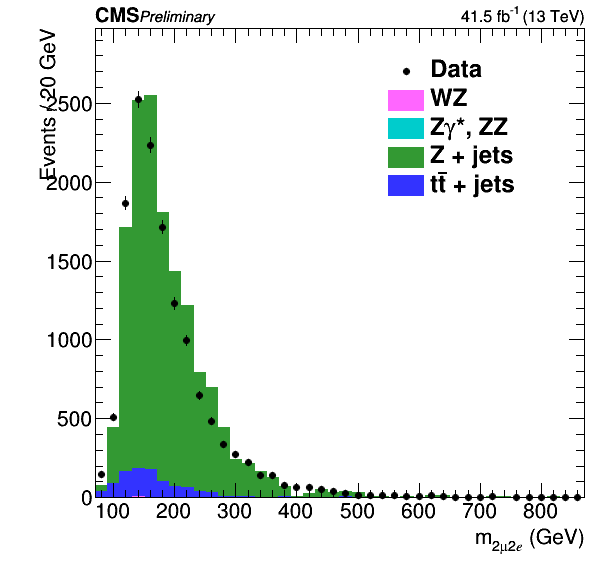
\includegraphics[width=0.45\textwidth]{Figures/RedBkg/M4l_dataMC/M4l_OS_2P2F_2mu2e_2017_Inclusive.png}}
        \subfigure[]{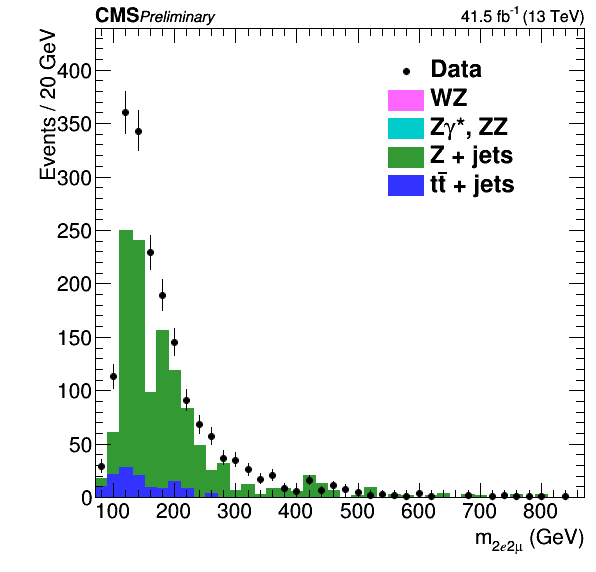
\includegraphics[width=0.45\textwidth]{Figures/RedBkg/M4l_dataMC/M4l_OS_2P2F_2e2mu_2017_Inclusive.png}} \\
\caption{
Invariant mass distribution of the events selected in the 2P+2F control sample in the
2017 dataset for all the considered channels: $4e$ (a), $4\mu$ (b), $2\mu2e$ (c) and $2e2\mu$ (d).
}
\label{fig:2P2F_dataMC2017}
\end{center}
\end{figure}

\begin{figure}[!htb]
\begin{center}
        \subfigure[]{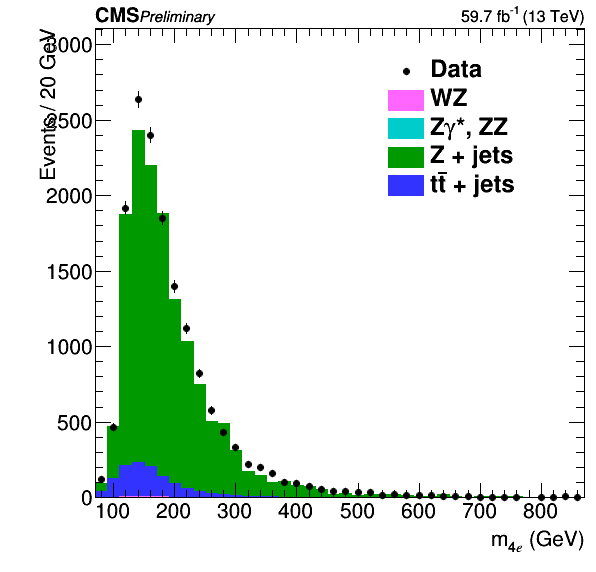
\includegraphics[width=0.45\textwidth]{Figures/RedBkg/M4l_dataMC/M4l_OS_2P2F_4e_2018_Inclusive.png}}
        \subfigure[]{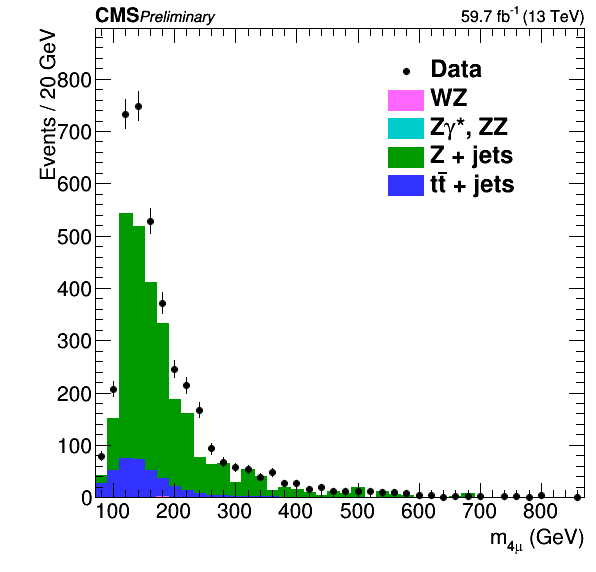
\includegraphics[width=0.45\textwidth]{Figures/RedBkg/M4l_dataMC/M4l_OS_2P2F_4mu_2018_Inclusive.png}}  \\
        \subfigure[]{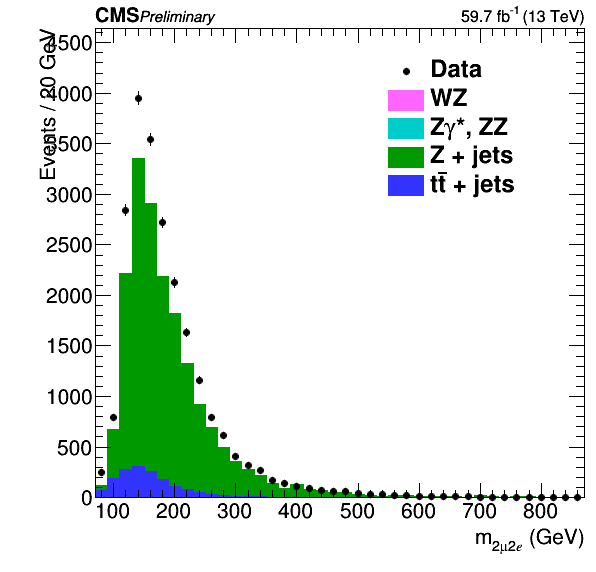
\includegraphics[width=0.45\textwidth]{Figures/RedBkg/M4l_dataMC/M4l_OS_2P2F_2mu2e_2018_Inclusive.png}}
        \subfigure[]{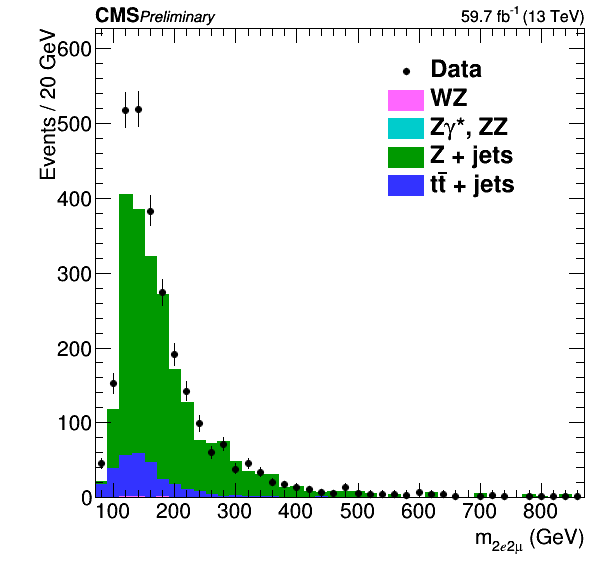
\includegraphics[width=0.45\textwidth]{Figures/RedBkg/M4l_dataMC/M4l_OS_2P2F_2e2mu_2018_Inclusive.png}} \\
\caption{
Invariant mass distribution of the events selected in the 2P+2F control sample in the
2018 dataset for all the considered channels: $4e$ (a), $4\mu$ (b), $2\mu2e$ (c) and $2e2\mu$ (d).
}
\label{fig:2P2F_dataMC2018}
\end{center}
\end{figure}


\begin{figure}[!htb]
\begin{center} 
        \subfigure[]{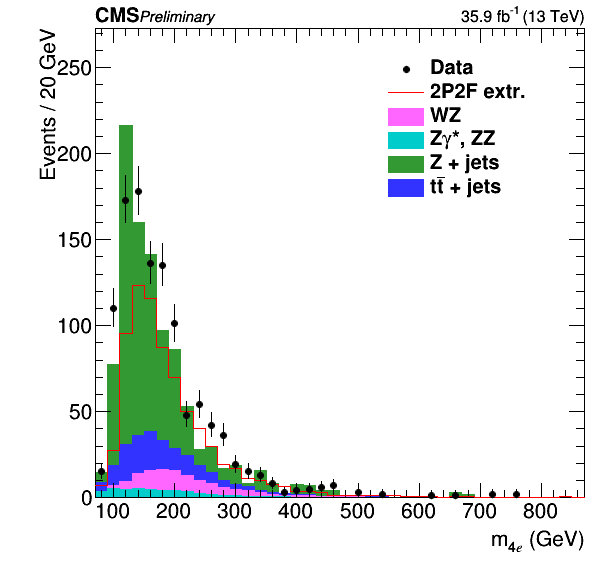
\includegraphics[width=0.45\textwidth]{Figures/RedBkg/M4l_dataMC/M4l_OS_3P1F_4e_2016_Inclusive.png}}
        \subfigure[]{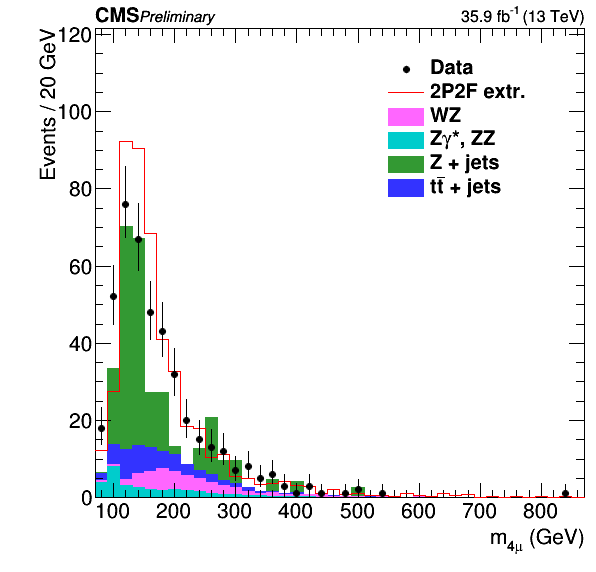
\includegraphics[width=0.45\textwidth]{Figures/RedBkg/M4l_dataMC/M4l_OS_3P1F_4mu_2016_Inclusive.png}}  \\
        \subfigure[]{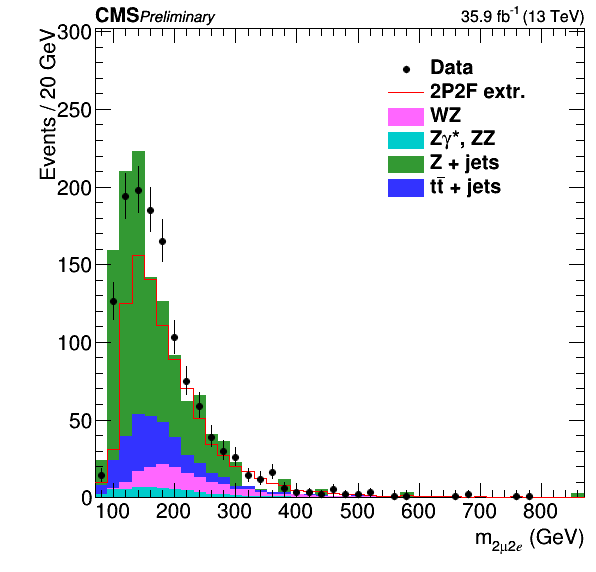
\includegraphics[width=0.45\textwidth]{Figures/RedBkg/M4l_dataMC/M4l_OS_3P1F_2mu2e_2016_Inclusive.png}}
        \subfigure[]{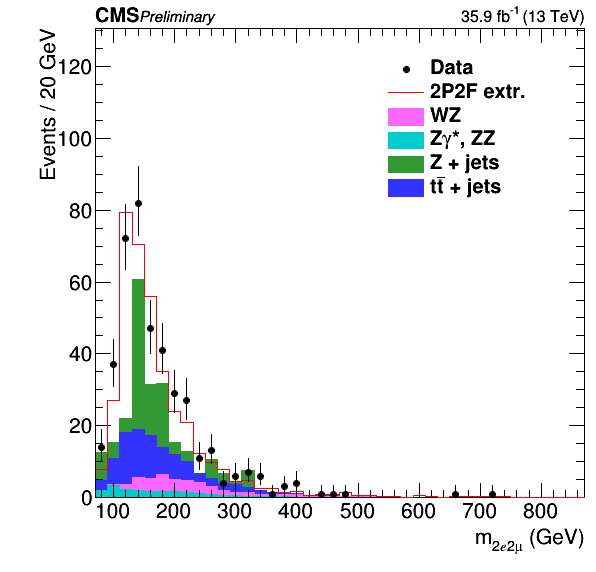
\includegraphics[width=0.45\textwidth]{Figures/RedBkg/M4l_dataMC/M4l_OS_3P1F_2e2mu_2016_Inclusive.png}} \\       
\caption{
Invariant mass distribution of the events selected in the 3P+1F control sample in the
2016 dataset for all the considered channels: $4e$ (a), $4\mu$ (b), $2\mu2e$ (c) and $2e2\mu$ (d).
}
\label{fig:CR_3P1F2016}
\end{center}
\end{figure}

\begin{figure}[!htb]
\begin{center} 
        \subfigure[]{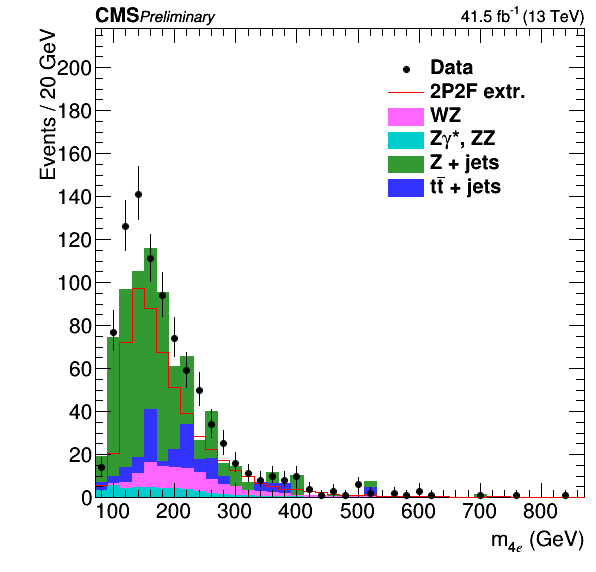
\includegraphics[width=0.45\textwidth]{Figures/RedBkg/M4l_dataMC/M4l_OS_3P1F_4e_2017_Inclusive.png}}
        \subfigure[]{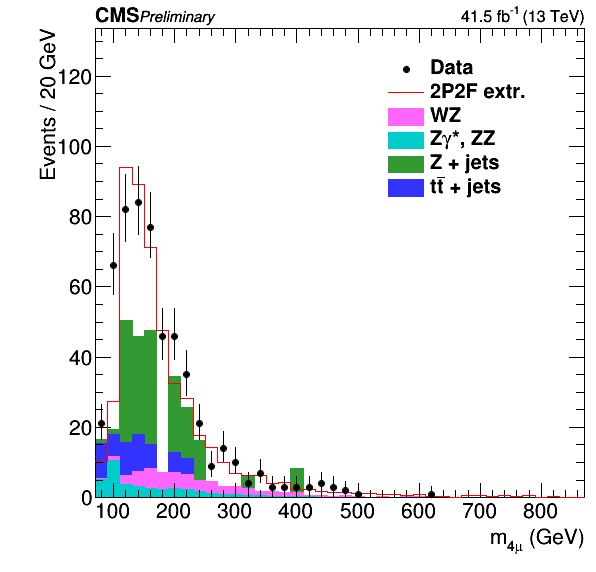
\includegraphics[width=0.45\textwidth]{Figures/RedBkg/M4l_dataMC/M4l_OS_3P1F_4mu_2017_Inclusive.png}}  \\
        \subfigure[]{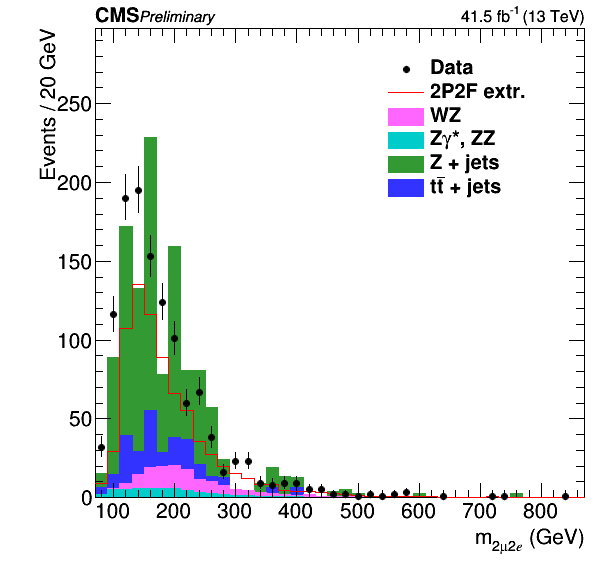
\includegraphics[width=0.45\textwidth]{Figures/RedBkg/M4l_dataMC/M4l_OS_3P1F_2mu2e_2017_Inclusive.png}}
        \subfigure[]{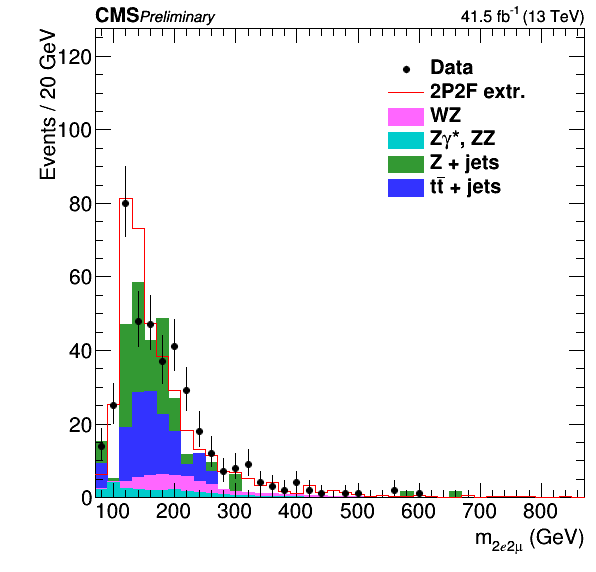
\includegraphics[width=0.45\textwidth]{Figures/RedBkg/M4l_dataMC/M4l_OS_3P1F_2e2mu_2017_Inclusive.png}} \\       
\caption{
Invariant mass distribution of the events selected in the 3P+1F control sample in the
2017 dataset for all the considered channels: $4e$ (a), $4\mu$ (b), $2\mu2e$ (c) and $2e2\mu$ (d).
}
\label{fig:CR_3P1F2017}
\end{center}
\end{figure}

\begin{figure}[!htb]
\begin{center} 
        \subfigure[]{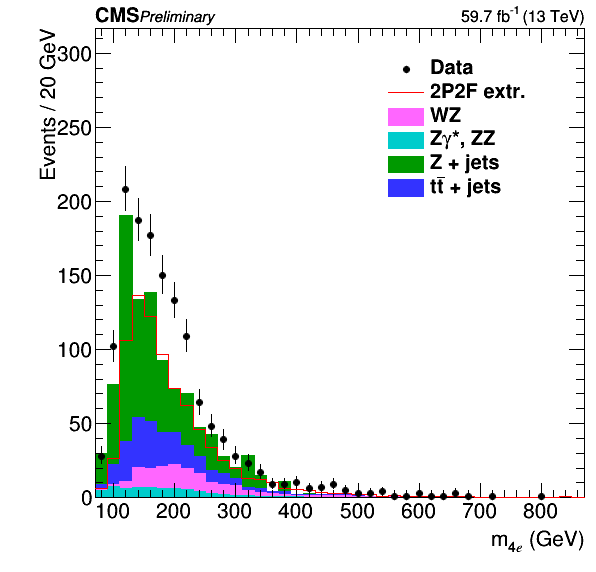
\includegraphics[width=0.45\textwidth]{Figures/RedBkg/M4l_dataMC/M4l_OS_3P1F_4e_2018_Inclusive.png}}
        \subfigure[]{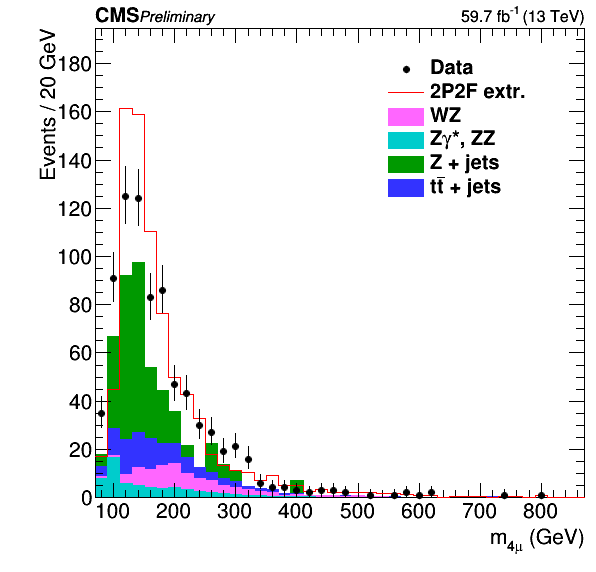
\includegraphics[width=0.45\textwidth]{Figures/RedBkg/M4l_dataMC/M4l_OS_3P1F_4mu_2018_Inclusive.png}}  \\
        \subfigure[]{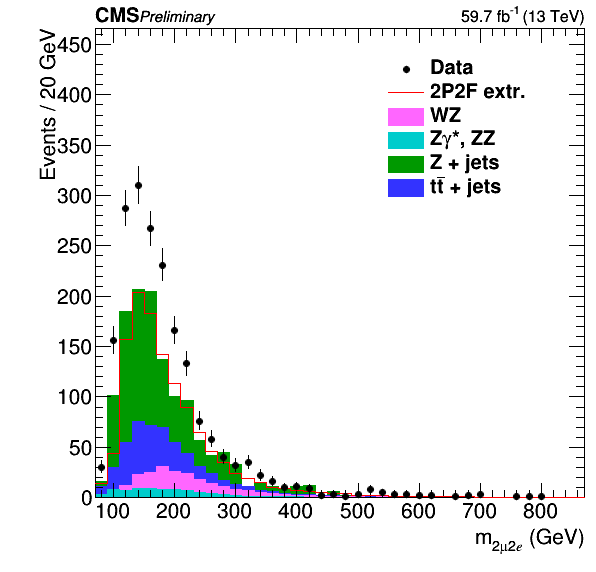
\includegraphics[width=0.45\textwidth]{Figures/RedBkg/M4l_dataMC/M4l_OS_3P1F_2mu2e_2018_Inclusive.png}}
        \subfigure[]{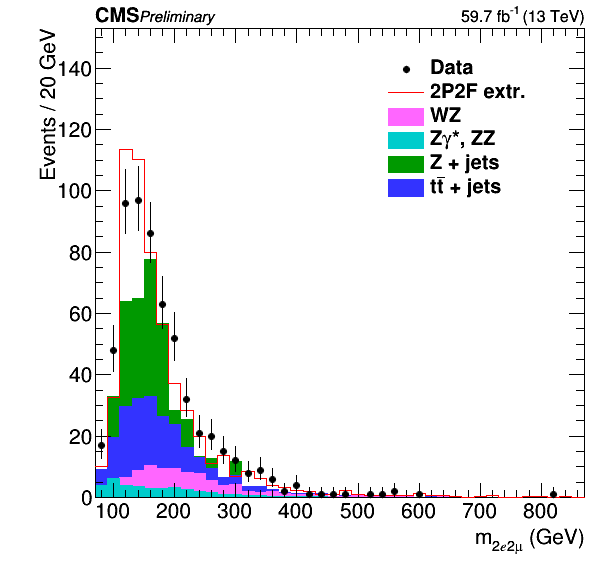
\includegraphics[width=0.45\textwidth]{Figures/RedBkg/M4l_dataMC/M4l_OS_3P1F_2e2mu_2018_Inclusive.png}} \\       
\caption{
Invariant mass distribution of the events selected in the 3P+1F control sample in the
2018 dataset for all the considered channels: $4e$ (a), $4\mu$ (b), $2\mu2e$ (c) and $2e2\mu$ (d).
}
\label{fig:CR_3P1F2018}
\end{center}
\end{figure}

The expected number of reducible background events in the 3P+1F region,
$N^{\rm bkg}_{\rm 3P1F}$, can be computed from the number of events
observed in the 2P+2F control region, $N_{\rm 2P2F}$, by weighting each
event in the region with the factor $(\frac{f_{i}}{1-f_{i}}
+ \frac{f_{j}}{1-f_{j}})$, where $f_{i}$ and $f_{j}$ correspond to the
fake ratios of the two loose leptons:

\begin{equation} 
\label{eq:Prediction3P1F}
N^{\rm bkg}_{\rm 3P1F} = \sum (\frac{f_{i}}{1-f_{i}}
+ \frac{f_{j}}{1-f_{j}}) N_{\rm 2P2F}
\end{equation} 

Figures~\ref{fig:CR_3P1F2016},~\ref{fig:CR_3P1F2017} and~\ref{fig:CR_3P1F2018} shows the invariant mass distributions of the
events selected in the 3P+1F control sample, together with the expected
reducible background estimated from Eq.~\ref{eq:Prediction3P1F},
stacked on the distribution
of $WZ$ and of irreducible background ($ZZ, Z\gamma* \to 4\ell$) taken from the simulation.

Would the fake rates be measured in a sample that has exactly the same
background composition as the 2P+2F sample, the difference between the
observed number of events in the 3P+1F sample and the expected background
predicted from the 2P+2F sample would solely amount to the (small) $WZ$ and $Z\gamma_{conv}$
contribution. Large differences arise because the fake rates used in
Eq.~\ref{eq:Prediction3P1F} do not properly account for the background
composition of the 2P+2F control sample.


In particular, the  difference seen in Figure~\ref{fig:CR_3P1F2018} between the observed
3P+1F distribution and the expectation from 2P+2F, in the
channels with loose electrons ($4e$ and $2\mu2e$), and concentrated at low
masses, is due to photon conversions. This is confirmed explicitly by the
simulation.
% : Figure~\ref{fig:CR_3P1F}c shows how events with a real photon populate
% this low mass region. Indeed, as the fake rates of method A are measured
% in a sample that is largely devoid of photon conversions, Eq.~\ref{eq:Prediction3P1F}
% considerably underestimates their contribution to the 3P+1F sample. 
%
The difference between the 3P+1F observation and the prediction
from 2P+2F to recover the missing contribution from conversions - and more generally,
in principle, to ``correct" for the fact that the fake rates do not properly
account for the background composition of the 2P+2F sample.
More precisely, the expected reducible background in the signal region is given
by the sum of two terms :
%
\begin{itemize}
\item a ``2P2F component", obtained from the number of
  events observed in the 2P+2F control region, $N_{\rm 2P2F}$, by
  weighting each event in that region with the factor
  $\frac{f_{i}}{1-f_{i}} \frac{f_{j}}{1-f_{j}}$, where $f_{i}$ and
  $f_{j}$ correspond to the fake ratios of the two loose leptons;
\item a ``3P1F component", obtained from the
   difference between the number of observed events in the 3P+1F control
   region, $N_{\rm 3P1F}$, and the expected contribution from the 2P+2F
   region and ZZ processes in the signal region, $N^{\rm ZZ}_{\rm 3P1F} +
   N^{\rm bkg}_{\rm 3P1F}$. The $N^{\rm bkg}_{\rm 3P1F}$ is given by 
   Eq. \ref{eq:Prediction3P1F} and $N^{\rm ZZ}_{\rm 3P1F}$ is the
   contribution from $ZZ$ which is taken from the simulation. 
   The difference $N_{\rm 3P1F} -  N^{\rm bkg}_{\rm 3P1F} - N^{\rm ZZ}_{\rm 3P1F}$,
   which may be negative,
   is obtained for each $(p_T, \eta)$ bin of the ``F" lepton, and is weighted 
   by $\frac{f_i} {1 - f_i}$, where $f_i$ denotes the fake rate of
   this lepton.
   This ``3P1F component" accounts for the contribution of reducible background
   processes with only one fake lepton (like $WZ$ events), and for the contribution
   of other processes (e.g. photon conversions) that are not properly estimated
   by the 2P2F component, because of the fake rates used.
\end{itemize}

Therefore, the full expression for the prediction can be symbolically written as:
%
\begin{equation} 
\label{eq:PredictionSR}
N^{bkg}_{\rm SR} = \sum \frac{f_{i}}{(1-f_{i})} (N_{\rm 3P1F} - N^{\rm
bkg}_{\rm 3P1F} - N^{\rm ZZ}_{\rm 3P1F})
+ \sum \frac{f_{i}}{(1-f_{i})} \frac{f_{j}}{(1-f_{j})}N_{\rm 2P2F} \end{equation}
%a
Previous equation is equivalent to the following:
\begin{equation}
\label{eq:PredictionSR2}
N^{bkg}_{\rm SR}= (1-\frac{N_{3P1F}^{ZZ}}{N_{3P1F}})\sum_j^{N_{3P1F}}\frac{f_a^j}{1-f_a^j} - \sum_i^{N_{2P2F}}\frac{f_3^i}{1-f_3^i}\frac{f_4^i}{1-f_4^i}
\end{equation}
For channels where the $Z_2$ candidate is made from two electrons, 
the contribution of the 3P1F component is 
positive, and amounts to typically $30 \%$ of the total predicted background.

For channels with loose muons ($4\mu$ and $2e2\mu$), the 3P+1F sample is rather well described by
the prediction from 2P+2F, as seen in Figure~\ref{fig:CR_3P1F2018}, and the
3P1F component is mainly driven by statistical fluctuations in the 3P+1F sample,
which are larger than the expectation from $WZ$ production.


%%%%%%%%%%%%%%%%%%%%%%%
Table~\ref{tab:reducibleMethodA} shows the expected number of
events in the signal regions from the reducible background processes at $13$~TeV for each considered final state and for all three years using the OS method.
%The uncertainty is given by the combination of a statistical uncertainty, which is dominated by the large statistical uncertainty of the ``3P1F" component, 
%and a systematic uncertainty due to the statistical uncertainty of the fake rates.
The invariant mass distribution of the ZX events obtained from the combination of the results in the 2P+2F and 3P+1F control samples
are shown in Figure~\ref{fig:combOS_dataMC2016},~\ref{fig:combOS_dataMC2017},~\ref{fig:combOS_dataMC2018}.
\begin{figure}[!htb]
\begin{center}
        \subfigure[]{\includegraphics[width=0.45\textwidth]{Figures/RedBkg/M4l_dataMC/M4l_OS_4e_2016-Inclusive.png}}
        \subfigure[]{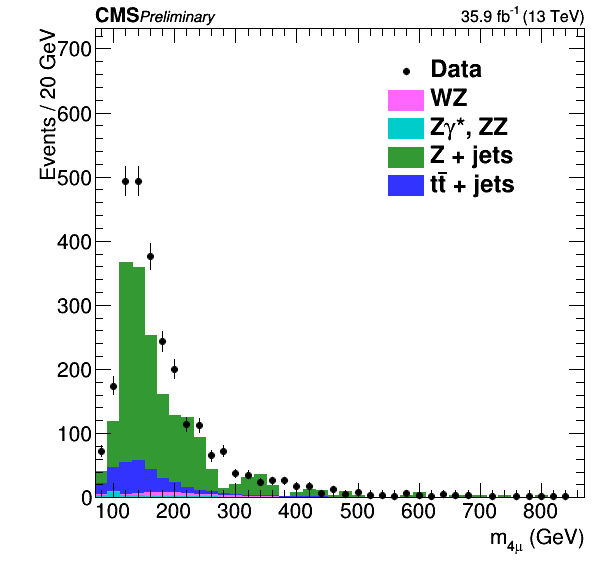
\includegraphics[width=0.45\textwidth]{Figures/RedBkg/M4l_dataMC/M4l_OS_4mu_2016_Inclusive.png}}  \\
        \subfigure[]{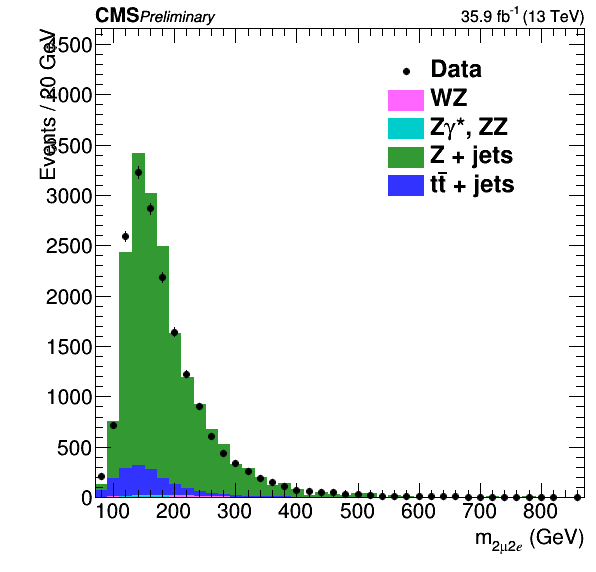
\includegraphics[width=0.45\textwidth]{Figures/RedBkg/M4l_dataMC/M4l_OS_2mu2e_2016_Inclusive.png}}
        \subfigure[]{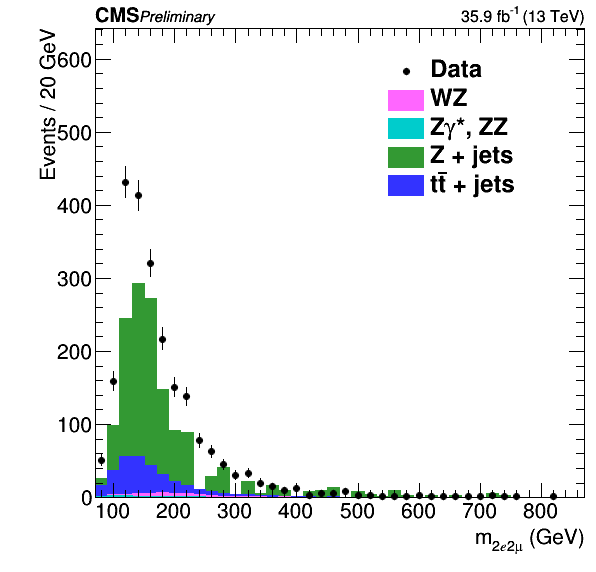
\includegraphics[width=0.45\textwidth]{Figures/RedBkg/M4l_dataMC/M4l_OS_2e2mu_2016_Inclusive.png}} \\       
\caption{
Invariant mass distribution of the events selected in the 2P+2F and 3P+1F control samples in the
2018 dataset for all the considered channels: $4e$ (a), $4\mu$ (b), $2\mu2e$ (c) and $2e2\mu$ (d) for 2016 data.
}
\label{fig:combOS_dataMC2016}
\end{center}
\end{figure}

\begin{figure}[!htb]
\begin{center}
        \subfigure[]{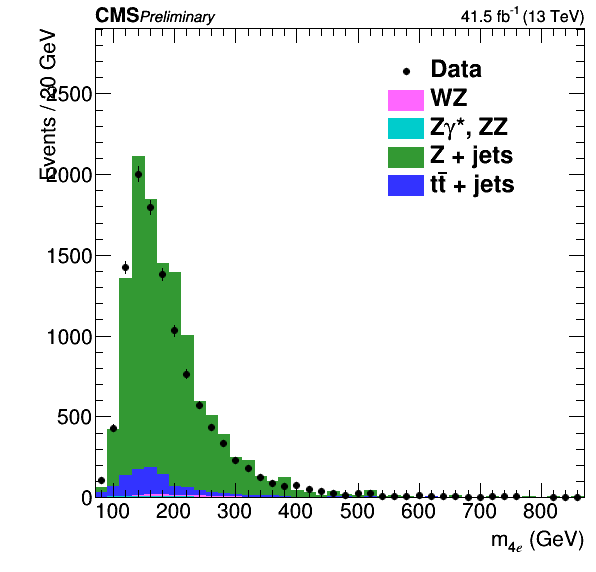
\includegraphics[width=0.45\textwidth]{Figures/RedBkg/M4l_dataMC/M4l_OS_4e_2017_Inclusive.png}}
        \subfigure[]{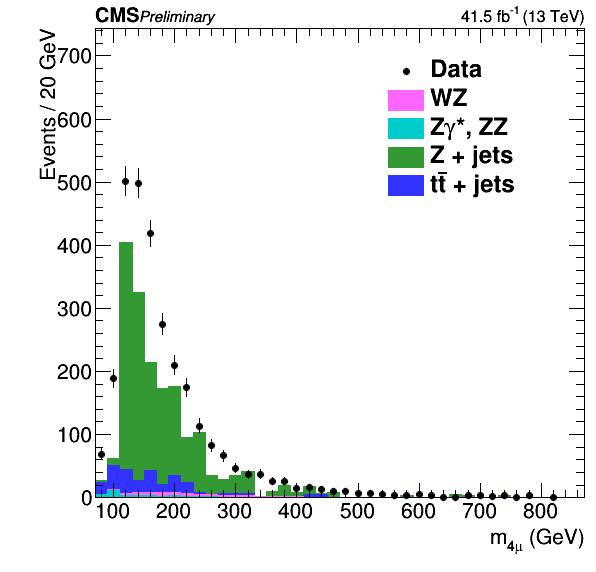
\includegraphics[width=0.45\textwidth]{Figures/RedBkg/M4l_dataMC/M4l_OS_4mu_2017_Inclusive.png}}  \\
        \subfigure[]{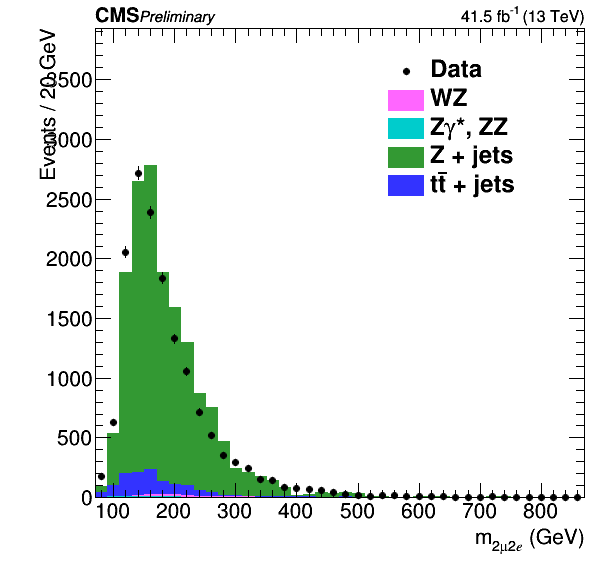
\includegraphics[width=0.45\textwidth]{Figures/RedBkg/M4l_dataMC/M4l_OS_2mu2e_2017_Inclusive.png}}
        \subfigure[]{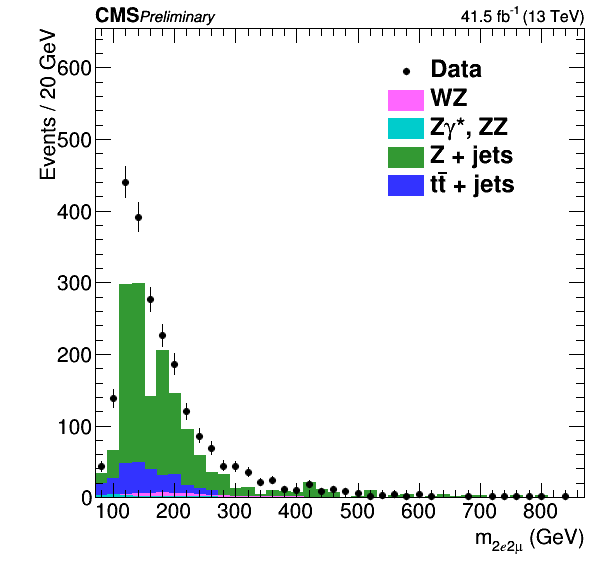
\includegraphics[width=0.45\textwidth]{Figures/RedBkg/M4l_dataMC/M4l_OS_2e2mu_2017_Inclusive.png}} \\       
\caption{
Invariant mass distribution of the events selected in the 2P+2F and 3P+1F control samples in the
2018 dataset for all the considered channels: $4e$ (a), $4\mu$ (b), $2\mu2e$ (c) and $2e2\mu$ (d) for 2017 data.
}
\label{fig:combOS_dataMC2017}
\end{center}
\end{figure}

\begin{figure}[!htb]
\begin{center}
        \subfigure[]{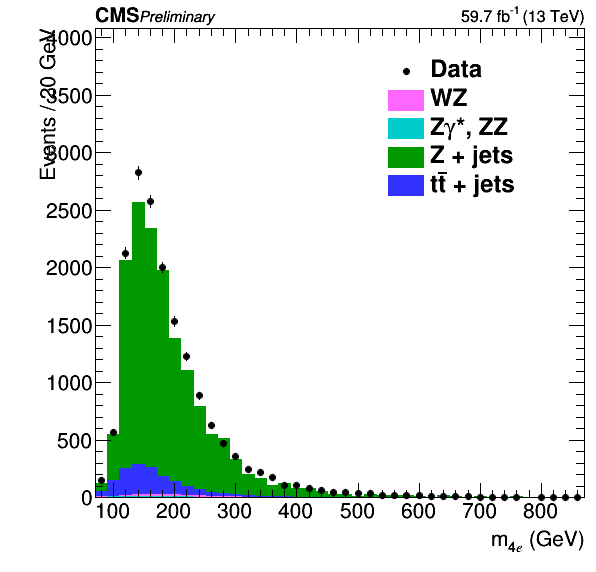
\includegraphics[width=0.45\textwidth]{Figures/RedBkg/M4l_dataMC/M4l_OS_4e_2018_Inclusive.png}}
        \subfigure[]{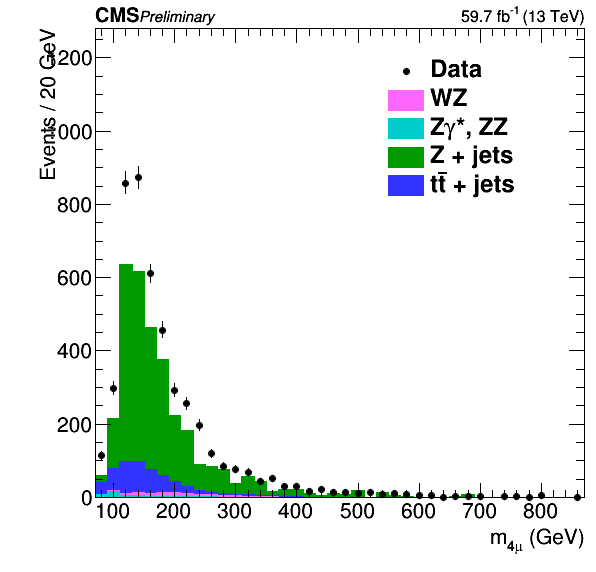
\includegraphics[width=0.45\textwidth]{Figures/RedBkg/M4l_dataMC/M4l_OS_4mu_2018_Inclusive.png}}  \\
        \subfigure[]{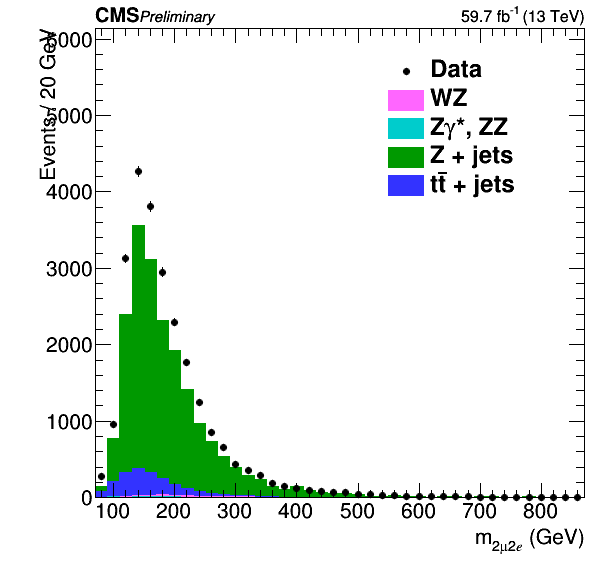
\includegraphics[width=0.45\textwidth]{Figures/RedBkg/M4l_dataMC/M4l_OS_2mu2e_2018_Inclusive.png}}
        \subfigure[]{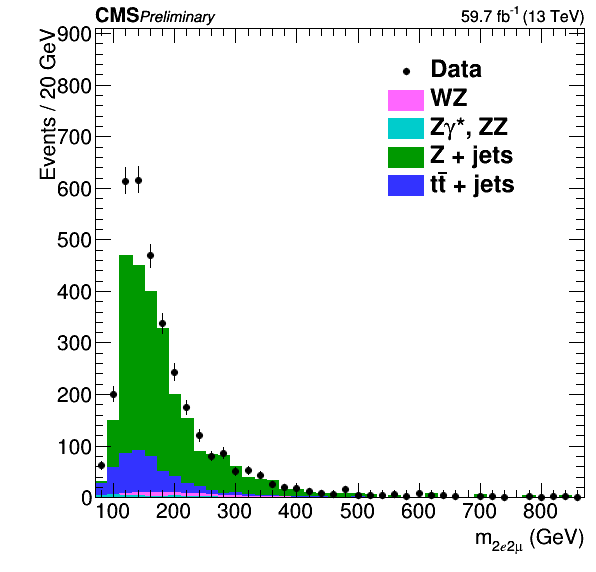
\includegraphics[width=0.45\textwidth]{Figures/RedBkg/M4l_dataMC/M4l_OS_2e2mu_2018_Inclusive.png}} \\       
\caption{
Invariant mass distribution of the events selected in the 2P+2F and 3P+1F control samples in the
2018 dataset for all the considered channels: $4e$ (a), $4\mu$ (b), $2\mu2e$ (c) and $2e2\mu$ (d) for 2018 data.
}
\label{fig:combOS_dataMC2018}
\end{center}
\end{figure}



\begin{table}[h]
\begin{center}
     \begin{tabular}{| l | c | c | c | c |} \hline
Channel	& 4e 	           & 4$\mu$          & 2e2$\mu$        & 2$\mu$2e        \\ \hline \hline
2016    & $ 20.1 \pm 6.1 $ & $26.9 \pm 8.6$ & $25.2 \pm 8.0$  & $22.3 \pm 6.8$  \\ 
2017    & $ 16.2 \pm 5.0 $ & $32.7 \pm 10.3$ & $24.0 \pm 7.7$  & $21.3 \pm 6.5$  \\ 
2018    & $ 25.4 \pm 7.7 $ & $49.4 \pm 15.4$ & $34.2 \pm 10.7$ & $33.0 \pm 10.0$ \\ \hline 
 	\end{tabular}
\end{center}
    \caption{ The contribution of reducible background
    processes in the signal region predicted from measurements in 2016, 2017 and 2018 data
    using the OS method. The predictions correspond to 35.9, 41.5 and 59.7~fb$^{-1}$ of data at $13$~TeV, respectively.}
     \label{tab:reducibleMethodA}
\end{table}


% SS method

\clearpage

\subsubsection{Reducible Background Estimate with Same-Sign Leptons}
\label{sec:zxSS}

This method used to predict the reducible background allows to
have an inclusive measurement of the all the main reducible
backgrounds at the same time.

The control sample is obtained as a subset of the events that satisfy
the first step of the selection ({\it First Z} step, see
section~\ref{sec:zzcandsel}), requiring an additional pair of 
loose leptons of same sign (to avoid signal contamination) and same
flavour (SS-SF: $e^{\pm}e^{\pm}, \mu^{\pm}\mu^{\pm}$).  The SS-SF
leptons are requested to pass the ${\rm SIP_{3D}}$, dxy and dz cuts, while no
identification requirements are imposed.  The
reconstructed invariant mass of the SS-SF leptons has to satisfy 
$m_{ \ell \ell} > 12$~GeV, $m_{ \ell \ell} < 120$~GeV,
the reconstructed four-lepton
invariant mass is required to satisfy $m_{4\ell} > 100~\GeVcc$,
and the QCD suppression cut (see~\ref{sec:zzcandsel}) is applied.
The inclusive number of reducible background events in the
signal region is derived from this set of events and from the probability for the
two additional leptons to pass the isolation and identification
analysis cuts, obtained from the fake rate measurement presented in section~\ref{sec:fakerate}.

Starting from the control sample previously described, the final
reducible background prediction in the signal region is given by the
following expression:
\begin{equation} 
\label{eq:FakeRateAA}
\begin{array}{cccc}
N^{\rm Z+X}_{\rm expect}  = & N^{\rm DATA}  \times   \rm{(\frac {OS}{SS})^{MC}}   \times &  
 f_1 \times f_2 
\end{array} 
\end{equation} 
where:
%
\begin{itemize}
\item $N^{\rm DATA}$ is the number of events in the control region,
\item $\rm{(\frac {OS}{SS})^{MC}}$ is a correction factor between opposite sign and same sign control samples,
\item $f_1$ and $f_2$ are the fake rates of each additional loose lepton, parameterised as a
   function of $p_T$ and $\eta$.
\end{itemize}

% ===============================================================================================================
%  FAKE RATE DETERMINATION
% ===============================================================================================================

\paragraph{Fake Rate Determination (SS method)}
\label{sec:fakerate}

The lepton fake rates are determined in the very similar way as it was described before for the OS method. Samples of $Z(\ell\ell)+e$ and $Z(\ell\ell)+\mu$ events are selected in the same way except that the mass window around the nominal Z mass is set to 40~GeV $< M_{inv}(\ell_{1},\ell_{2}) < $ 120~GeV, as in the signal region ("SS phase space").
Despite the cut on the missing transverse energy, a contamination of real leptons from WZ events is still visible at high $p_T$. This contribution is thus subtracted from the final fake rate, using the estimation given by the Monte Carlo. The fake rates for muon are shown in Figure~\ref{fig:fakerates} for both muons in the barrel ($|\eta|<1.2$) and in the endcaps ($|\eta|>1.2$).

%=======  
\begin{figure}[!htb]
\begin{center}
    \subfigure [] {\resizebox{5.1cm}{!}{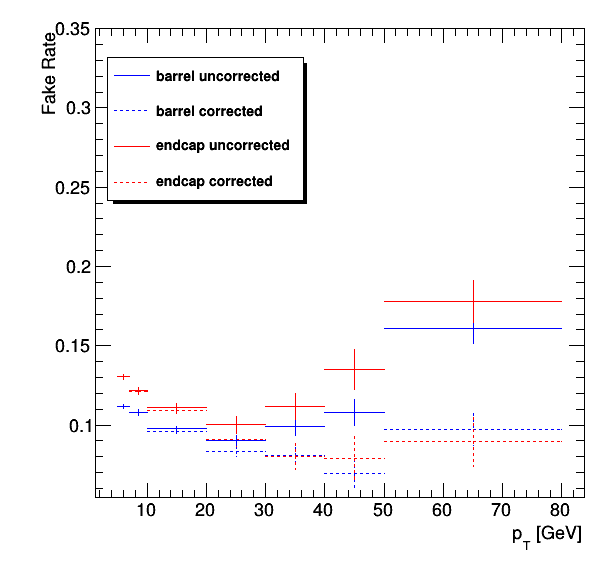
\includegraphics{Figures/RedBkg/FR/FR_SS_muons_2016.png}}}
    \subfigure [] {\resizebox{5.1cm}{!}{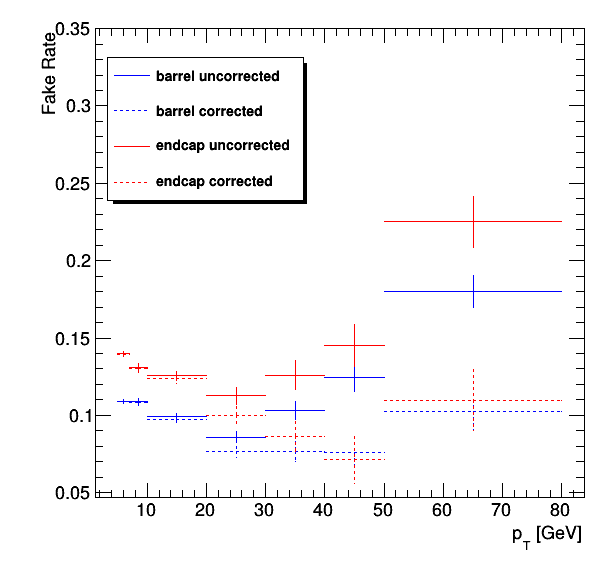
\includegraphics{Figures/RedBkg/FR/FR_SS_muons_2017.png}}}
    \subfigure [] {\resizebox{5.1cm}{!}{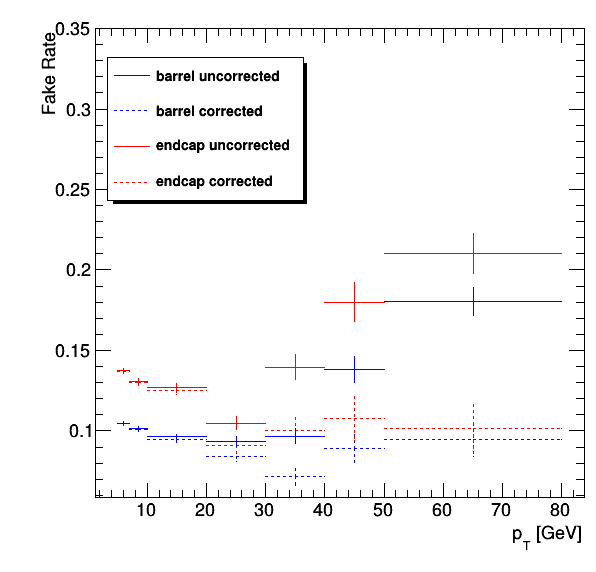
\includegraphics{Figures/RedBkg/FR/FR_SS_muons_2018.png}}}
\caption{Fake rates as a function of the probe $p_T$ for muons which satisfy the loose selection criteria, measured in
a $Z(\ell\ell)+\ell$ sample in the 2016 (top), 2017 (middle) and 2018 (bottom) data at $13$~TeV.
The barrel selection includes electrons (muons) up to $|\eta|$ = 1.479 (1.2). The fake rates are shown before (dotted lines) and after (plain line) the removal of the WZ contribution from the simulation.
}
\label{fig:fakerates}
\end{center}
\end{figure}
%=======  

For electrons, events where a radiated photon makes an asymmetric conversion, where one low $p_T$ leg is not identified, contribute to the $Z + e$ sample that is used to measure the electron fake rate. While the requirement $|M_{inv}(\ell_{1},\ell_{2}) - M_{Z}| < 7 $~GeV ("OS phase space") largely suppresses FSR of photons radiated off the lepton legs, these radiations occur at a much larger rate in the "SS phase space". 
As a result of this enhanced
contribution from conversions, the electron fake rates measured
within the SR phase space  are larger than the "OS fake rates".

However, the relative fraction of FSR conversions is not the same in the "SS phase space"
and in the control sample (defined below) where the fake rates will be applied. A correction
accounting for this difference must be applied to the fake rates measured within 
the SS phase space, in order to obtain
average fake rates that are appropriate for the control sample.
To determine this correction,
several fake rate samples of $Z(ll) + e$ events are defined by applying different 
cuts on $M_{inv}(\ell_{1},\ell_{2})$ or on $M_{inv}(\ell_{1},\ell_{2}, e)$.
In addition to the "OS fake rate sample", where $|M_{inv}(\ell_{1},\ell_{2}) - M_{Z}| < 7 $~GeV ensures
a minimal amount of conversions from FSR photons, one defines a sample that is
maximally enriched in FSR conversions by
$ | M_{inv}(\ell_{1},\ell_{2}, e) - M_Z | < $~5~GeV,
as well as samples with 
an intermediate contamination from FSR conversions (60~GeV $< M_{inv}(\ell_{1},\ell_{2}) < $ 120~GeV).
In each sample, one determines in several $(p_T, \eta)$ bins for the loose electron:
\begin{itemize}
 \item the fake rate ratio;
 \item the average value of the expected inner missing hits ($N_{miss. hits}$ in the following), variable useful to tag conversions. 
\end{itemize}
%

In a given $(p_T, \eta)$  bin, both the measured fake rate and the
average $ < N_{miss. hits} > $ are expected to grow linearly with the fraction
of conversions. 
Hence, one expects a linear dependence of the fake rate with respect to $ < N_{miss. hits} > $.
This linear behaviour is demonstrated in Figure~\ref{fig:FRvsNHits}, and linear fits are made
in each $(p_T, \eta)$  bin, which relate the fake rate to $ < N_{miss. hits} > $.
Finally, one looks at the loose electrons in the control sample where the fake rate will be applied, 
and $<N_{miss. hits}>$ is measured in each $(p_T, \eta)$ bin.
The proper average fake rate corresponding to the control sample is then determined from the
linear relation derived previously.
Figure~\ref{fig:FRAAcorrected} shows examples of the resulting corrected fake rates, together with the
fake rates measured in the SS phase space.
It can be seen that the correction for the actual fraction of conversions that is present in the
control sample lowers the fake rates considerably with respect to what is measured
in the SS phase space.
The determination of these corrected fake rates mostly suffers from the limited statistics of the
control sample, which translates into a large uncertainty on $<N_{miss. hits}>$, 
the error on each dot being the fake rate obtained from the linear relations using the error on the $<N_{miss. hits}>$.

\begin{figure}[!h]
\begin{center}
    \subfigure [] {\resizebox{7.75cm}{!}{\includegraphics{Figures/RedBkg/FR_MissingHits_graph_eta_0_pT_0.png}}} 
    \subfigure [] {\resizebox{7.75cm}{!}{\includegraphics{Figures/RedBkg/FR_MissingHits_graph_eta_1_pT_4.png}}} 
\caption{
Examples of the correlation between the fake rate and the fraction of loose electrons 
for which the track has one missing hit in the pixel detector for  $7<p_T<10$~GeV electrons in the barrel (left) and for $30<p_T<40$~GeV electrons in the endcaps (right).
Each dot shows the measurements made in a given $Z$ + loose $e$ sample.
Results are produced at 13~TeV with 35.9~fb$^{-1}$ data.
}
\label{fig:FRvsNHits}
\end{center}
\end{figure}

%=======  
\begin{figure}[!htb]
\begin{center}
    \subfigure [] {\resizebox{5.1cm}{!}{\includegraphics{Figures/RedBkg/FR/FR_SS_electrons_2016.png}}}
    \subfigure [] {\resizebox{5.1cm}{!}{\includegraphics{Figures/RedBkg/FR/FR_SS_electrons_2017.png}}}
    \subfigure [] {\resizebox{5.1cm}{!}{\includegraphics{Figures/RedBkg/FR/FR_SS_electrons_2018.png}}}
\caption{Average fake rates to be applied to the control sample of SS method (plain line), compared to
  the fake rates measured in the SS phase space (dotted line), for electrons in the barrel (blue) and in the endcaps (red).
  Results are produced at 13~TeV with 2016, 2017, and 2018 data.
}
\label{fig:FRAAcorrected}
\end{center}
\end{figure}
%=======  

% ============================================================================================================
%  FAKE RATE APPLICATION
% ============================================================================================================
\paragraph{Fake Rate Application (SS method)}
Figure~\ref{fig:ZjetControlRegionShapes13TeV} shows the invariant mass
distribution of events in control samples with SS-SF loose leptons,
for channels with loose electrons ($4e$ and $2\mu2e$) and channels
with loose muons ($4\mu$ and $2e2\mu$), for the 2018 dataset at $13$~TeV. 
The prediction from the Monte Carlo simulation is also shown.

A good agreement is achieved between data and MC for the channels
with loose electrons. The agreement is not as good for loose muons
but this has no impact on the final result as only data are used in the end.  

The differences in rates between OS and SS samples are estimated using data and are used to compute 
the correction factor in Eq.~\ref{eq:FakeRateAA} for the final data-driven estimation. 
They are given for each year in Table~\ref{tab:OSSS}.

\begin{table}[!htb]
% \scriptsize
\begin{center}
    \begin{tabular}{ | l | c | c | c |  c | }  \hline
   Channel  &  4e               &  2$\mu$2e          &  4$\mu$           &  2e2$\mu$        \\ \hline \hline   
   2016     &  1.00 $\pm$ 0.01  &  1.00 $\pm$ 0.01   &  1.00 $\pm$ 0.03  &  1.00 $\pm$ 0.03 \\ 
   2017     &  1.01 $\pm$ 0.01  &  1.00 $\pm$ 0.01   &  1.04 $\pm$ 0.03  &  1.01 $\pm$ 0.03 \\ 
   2018     &  1.01 $\pm$ 0.01  &  1.00 $\pm$ 0.01   &  1.03 $\pm$ 0.02  &  1.03 $\pm$ 0.02 \\ \hline
    \end{tabular}
    \caption{ The OS/SS ratios used to estimate the number of ZX events with the SS method for each final state in all three years. }
    \label{tab:OSSS}
\end{center}
\end{table}

%=======  
\begin{figure}[!h]
\begin{center}
\subfigure[]{\includegraphics[width=0.45\textwidth]{Figures/RedBkg/M4l_dataMC/M4l_SS_4e_2018_Inclusive.png}} 
\subfigure[]{\includegraphics[width=0.45\textwidth]{Figures/RedBkg/M4l_dataMC/M4l_SS_4mu_2018_Inclusive.png}}  \\ 
\subfigure[]{\includegraphics[width=0.45\textwidth]{Figures/RedBkg/M4l_dataMC/M4l_SS_2mu2e_2018_Inclusive.png}}  
\subfigure[]{\includegraphics[width=0.45\textwidth]{Figures/RedBkg/M4l_dataMC/M4l_SS_2e2mu_2018_Inclusive.png}} \\ 
\caption{Invariant mass distribution of the events selected in the SS-SF control samples for all the considered final states in 2018 data:
$4e$ (a), $4\mu$ (b), $2\mu2e$ (c) and $2e2\mu$ (d).  
\label{fig:ZjetControlRegionShapes13TeV}}
\end{center}
\end{figure}
%=======  

The event yields expected from the Z+X in the signal region, in the mass range  $m_{4 \ell} > 70~\GeVcc$, are calculated for each final state.
%and for each of the 22 STXS Stage 1.1 categories defined in Section~\ref{sec:categorization}. An example for the $4e$ final state in 2018 data is shown in Table~\ref{tab:ZjetResultsAA_4e}.
%The statistical error is due to the event statistics in the control region, while the systematic one is due to error introduced with the missing hits based correction for electrons and the uncertanty in the fake rates in the muon case. 
The background is due to the systematic introduced when estimating the background composition. 
The total error is obtained with a quadrature sum for the statistical, background composition and correction systematics. 
Table~\ref{tab:SSyields} shows the expected number of events in the signal regions 
from the reducible background processes at $13$~TeV for each considered final state 
and for all three years using the SS method.
%
%
%\begin{table}[htb!]
%\begin{center}
%\small
%\begin{tabular}{ l | c | c | c | c | c | c}
%\hline
%\hline
%Category & exp. $N^{\rm Z+X}$ in SR & (stat.) & (syst. - FR) & (syst - Bkg comp) & Total unc.\\
%\hline
%\hline
%ggH\_0J\_PTH\_0\_10        & 0.35 & $\pm 0.02$ & $\pm 0.07 $    & $\pm 0.11 $  & $\pm 0.13 $ \\
%\hline
%ggH\_0J\_PTH\_10\_200      & 6.75 & $\pm 0.08$ & $\pm 1.40 $    & $\pm 2.03 $  & $\pm 2.48 $ \\
%\hline
%ggH\_1J\_PTH\_0\_60        & 2.18 & $\pm 0.04$ & $\pm 0.44 $    & $\pm 0.65 $  & $\pm 0.79 $ \\
%\hline
%ggH\_1J\_PTH\_60\_120      & 1.51 & $\pm 0.04$ & $\pm 0.32 $    & $\pm 0.45 $  & $\pm 0.56 $ \\
%\hline
%ggH\_1J\_PTH\_120\_200     & 0.53 & $\pm 0.02$ & $\pm 0.12 $    & $\pm 0.16 $  & $\pm 0.20 $ \\
%\hline
%ggH\_2J\_PTH\_0\_60        & 0.65 & $\pm 0.02$ & $\pm 0.13 $    & $\pm 0.20 $  & $\pm 0.23 $ \\
%\hline
%ggH\_2J\_PTH\_60\_120      & 0.74 & $\pm 0.03$ & $\pm 0.16 $    & $\pm 0.22 $  & $\pm 0.27 $ \\
%\hline
%ggH\_2J\_PTH\_120\_200     & 0.31 & $\pm 0.02$ & $\pm 0.07 $    & $\pm 0.09 $  & $\pm 0.12 $ \\
%\hline
%ggH\_PTH\_200              & 0.45 & $\pm 0.02$ & $\pm 0.11 $    & $\pm 0.14 $  & $\pm 0.17 $ \\
%\hline
%ggH\_VBF                   & 0.28 & $\pm 0.02$ & $\pm 0.06 $    & $\pm 0.08 $  & $\pm 0.10 $ \\
%\hline
%VBF\_1j                    & 0.47 & $\pm 0.02$ & $\pm 0.09 $    & $\pm 0.14 $  & $\pm 0.17 $ \\
%\hline
%VBF\_2j                    & 0.30 & $\pm 0.02$ & $\pm 0.06 $    & $\pm 0.09 $  & $\pm 0.11 $ \\
%\hline
%VBF\_2j\_mjj\_350\_700\_2j & 0.02 & $\pm 0.00$ & $\pm 0.00 $    & $\pm 0.01 $  & $\pm 0.01 $ \\
%\hline
%VBF\_2j\_mjj\_GT700\_2j    & 0.02 & $\pm 0.002$ & $\pm 0.003 $  & $\pm 0.01 $  & $\pm 0.01 $ \\
%\hline
%VBF\_2j\_mjj\_GT350\_3j    & 0.40 & $\pm 0.02$ & $\pm 0.09 $    & $\pm 0.12 $  & $\pm 0.15 $ \\
%\hline
%VBF\_GT200\_2J             & 0.03 & $\pm 0.01$ & $\pm 0.01 $    & $\pm 0.01 $  & $\pm 0.01 $ \\
%\hline
%VH\_Had                    & 0.57 & $\pm 0.02$ & $\pm 0.12 $    & $\pm 0.17 $  & $\pm 0.21 $ \\
%\hline
%VBF\_rest\_VH              & 0.10 & $\pm 0.01$ & $\pm 0.02 $    & $\pm 0.03 $  & $\pm 0.04 $ \\
%\hline
%VH\_lep\_0\_150            & 0.13 & $\pm 0.01$ & $\pm 0.03 $    & $\pm 0.04 $  & $\pm 0.05 $ \\
%\hline
%VH\_Lep\_GT150             & 0.01 & $\pm 0.00$ & $\pm 0.00 $    & $\pm 0.00 $  & $\pm 0.00 $ \\
%\hline
%ttH\_Lep                   & 0.04 & $\pm 0.01$ & $\pm 0.01 $    & $\pm 0.01 $  & $\pm 0.02 $ \\
%\hline
%ttH\_Had                   & 0.19 & $\pm 0.01$ & $\pm 0.04 $    & $\pm 0.06 $  & $\pm 0.07 $ \\
%\hline
%\hline
%Inclusive                  & 16.0 & $\pm 0.12$ & $\pm 3.34 $    & $\pm 4.8 $ & $\pm 5.85 $ \\
%\hline
%\hline
%\end{tabular}
%\end{center}
%\caption{Number of $4e$ events in the SS-SF control region for 59.7~fb$^{-1}$ of 2018 data, and expected number of Z+X$\to4\Pe$ events in the signal region as predicted from the SS method. The total uncertainty associated to the SS measurement is shown in the table together with the splitting in its three contributions: statistical error and both systematic errors due to fake rate variation and background composition.
%\label{tab:ZjetResultsAA_4e}}
%\end{table}
%

\begin{table}[!htb]
\begin{center}
     \begin{tabular}{| l | c | c | c | c |} \hline
Channel & 4e               & 4$\mu$          & 2e2$\mu$        & 2$\mu$2e        \\ \hline \hline
2016    & $ 13.0 \pm 5.4 $ & $29.7 \pm 9.1$  & $24.8 \pm 7.6$  & $16.7 \pm 7.0$  \\
2017    & $ 10.9 \pm 4.0 $ & $33.6 \pm 10.3$ & $26.3 \pm 8.1$  & $14.7 \pm 5.5$  \\
2018    & $ 16.0 \pm 5.9 $ & $52.2 \pm 15.8$ & $37.4 \pm 11.4$ & $23.3 \pm 8.5$  \\ \hline
        \end{tabular}
\end{center}
    \caption{ The contribution of reducible background
    processes in the signal region predicted from measurements in 2016, 2017 and 2018 data
    using the SS method. The predictions correspond to 35.9, 41.5 and 59.7~fb$^{-1}$ of data at $13$~TeV, respectively.}
     \label{tab:SSyields}
\end{table}

\paragraph{Fake Rate in the VBF-tagged categories}
The FR are currently evaluated inclusively in the analysis: in fact, an average fake rate is used to evaluate ZX yields in each STXS category instead of dedicated ones.
Given that the VBF category can be particularly affected by this approach, a detailed study of the FR variation in different Z+L phase spaces designed to mimic VBF has been performed using 2018 data. 
However, a realistic design of the VBF phase space is not completely reproducible in the three leptons CR without exploiting the information given by the kinematic discriminants.
In order to identify events targeting VBF-tagged categories, the following requirements on jets are applied:
\begin{itemize} 
\item an angular separation between the additional lepton and each jet larger than 0.4, otherwise the jet is discarded;       
\item the presence of two or three jets and at most one b tagged jet OR at least four jets without b tagged jets;
\item an angular separation between the pair of two leading jets larger than 0.5 and a dijet invariant mass greater than 450 GeV. 
\end{itemize}

Futhermore, FR in the CR Z+L with 0/1/2 jets have been studied as well as the FR in the phase space complementary to the VBF-like one.
Figure~\ref{fig:FRSSperCat} shows the FR curves obtained in each category for both electrons and muons in the barrel and endcap region using the SS method and Figure~\ref{fig:FROSperCat} shows the same distributions using the OS method. 
While the curve in the "non VBF-tagged'' region is perfectly in agreement with the inclusive one (as a result of the contribution of the 0/1/2 jet categories),   
the FR variation in the 0/1/2 jets and VBF-like categories is significant, especially for muons.
As a consequence, large discrepancies are observed in the final estimated yields in VBF categories (Table~\ref{tab:VBFyields}).

%=======  
\begin{figure}[!h]
\begin{center}
\subfigure[]{\includegraphics[width=0.45\textwidth]{Figures/RedBkg/FR/allCat_FR_muon_EB_2018_SS.png}} 
\subfigure[]{\includegraphics[width=0.45\textwidth]{Figures/RedBkg/FR/allCat_FR_muon_EE_2018_SS.png}}}  \\ 
\subfigure[]{\includegraphics[width=0.45\textwidth]{Figures/RedBkg/FR/allCat_FR_electron_EB_2018_SS.png}}}  
\subfigure[]{\includegraphics[width=0.45\textwidth]{Figures/RedBkg/FR/allCat_FR_electron_EE_2018_SS.png}}} \\ 
\caption{FR curves in the 0/1/2/VBF-tagged and non VBF-tagged categories for muons (top) and electrons (bottom) in the barrel (left) and endcap (right) region obtained using SS method.   
\label{fig:FRSSperCat}}
\end{center}
\end{figure}
%=======    
\begin{figure}[!h]
\begin{center}
\subfigure[]{\includegraphics[width=0.45\textwidth]{Figures/RedBkg/FR/allCat_FR_muon_EB_2018_OS.png}} 
\subfigure[]{\includegraphics[width=0.45\textwidth]{Figures/RedBkg/FR/allCat_FR_muon_EE_2018_OS.png}}}  \\ 
\subfigure[]{\includegraphics[width=0.45\textwidth]{Figures/RedBkg/FR/allCat_FR_electron_EB_2018_OS.png}}}  
\subfigure[]{\includegraphics[width=0.45\textwidth]{Figures/RedBkg/FR/allCat_FR_electron_EE_2018_OS.png}}} \\ 
\caption{FR curves in the 0/1/2/VBF-tagged and non VBF-tagged categories for muons (top) and electrons (bottom) in the barrel (left) and endcap (right) region obtained using OS method.   
\label{fig:FRSSperCat}}
\end{center}
\end{figure}
%=======  

\begin{table}[!h]
        \begin{center}
                \caption{
                Comparison between combined ZX yields in the VBF-tagged categories using inclusive and dedicated FR. 
                \label{tab:VBFyields}
                        }
    \renewcommand{\arraystretch}{1.5}
    \begin{tabular}{c|cccc|cccc}
        & \multicolumn{4}{c|}{Inclusive FR} & \multicolumn{4}{c}{Dedicated FR} \\
        CATEGORY                   & $4l$  & $4\mu$ & $4e$ & $2e2\mu$  & $4l$ & $4\mu$ & $4e$ & $2e2\mu$ \\
        \hline
        VBF\_1j                     & 1.047 & 0.391 & 0.147 & 0.509    & 0.663 & 0.185 & 0.113 & 0.365  \\
        VBF\_2j                     & 0.882 & 0.295 & 0.097 & 0.490    & 0.054 & 0.011 & 0.016 & 0.028  \\
        VBF\_2j\_mjj\_350\_700\_2j  & 0.040 & 0.026 & 0.003 & 0.011    & 0.004 & 0.000 & 0.000 & 0.004  \\
        VBF\_2j\_mjj\_GT700\_2j     & 0.016 & 0.013 & 0.002 & 0.001    & 0.091 & 0.018 & 0.039 & 0.034  \\
        VBF\_2j\_mjj\_GT350\_3j     & 0.997 & 0.444 & 0.104 & 0.450    & 0.001 & 0.001 & 0.000 & 0.000  \\
        VBF\_GT200\_2J              & 0.021 & 0.019 & 0.001 & 0.001    & 0.015 & 0.001 & 0.001 & 0.014  \\
        \hline                      
        Inclusive VBF               & 3.002 & 1.188 & 0.353 & 1.461    & 0.828 & 0.216 & 0.169 & 0.444  \\
        \hline


\end{tabular}
        \end{center}
\end{table}

In principle, the uncertainty on the background composition of the CR was designed to cover for this effect, but considering that the effect seems very large, 
the possible impact on the analysis has been checked explicitely. 
An extreme situation has been studied by inflating the Z+X uncertainty by 100$\%$ in the datacards in VBF-tagged categories and comparing stage 0 signal strengths, 
both expected and observed, using the standard Z+X uncertainty and inflating it in VBF categories (Table~\ref{tab:inflatedMu}). 
The results show that the expected uncertainty does not change and the observed signal strengths change only very slightly (2nd digit) within the uncertainties. 

\begin{table}[!h]
        \begin{center}
                \caption{
                Comparison between the best-fit values and $\pm 1\sigma$ uncertainties for the expected and observed signal-strength modifiers,
                inflating ZX uncertainties in VBF categories by 100$\%$ and keeping nominal ZX uncertainties.
                \label{tab:inflatedMu}
                        }
    \renewcommand{\arraystretch}{1.5}
    \begin{tabular}{c|cc|cc}
        & \multicolumn{2}{c|}{Inflated ZX uncertainty} & \multicolumn{2}{c}{Nominal ZX uncertainty} \\
        & Expected  & Observed & Expected & Observed \\
        \hline
        $\mu_{\ttH,\tH}$       & $1.00~^{+1.36}_{-0.78}~$ & $0.23 ^{+0.95}_{-0.23}$   & $1.00~^{+1.36}_{-0.78}~$ & $0.22 ^{+0.95}_{-0.22}$ \\
        $\mu_{\WH}$            & $1.00~^{+2.01}_{-1.00}~$ & $1.68 ^{+1.76}_{-1.44}$   & $1.00~^{+2.01}_{-1.00}~$ & $1.71 ^{+1.79}_{-1.71}$ \\
        $\mu_{\ZH}$            & $1.00~^{+8.33}_{-1.00}~$ & $0.00 ^{+5.24}_{-0.00}$   & $1.00~^{+8.33}_{-1.00}~$ & $0.00 ^{+5.44}_{-0.00}$ \\
        $\mu_{\mathrm{VBF}}$   & $1.00~^{+0.56}_{-0.46}~$ & $0.54 ^{+0.51}_{-0.41}$   & $1.00~^{+0.56}_{-0.46}~$ & $0.56 ^{+0.50}_{-0.41}$ \\
        $\mu_{\Pg\Pg\PH,\bbH}$ & $1.00~^{+0.16}_{-0.14}~$ & $1.02 ^{+0.15}_{-0.13}$   & $1.00~^{+0.16}_{-0.14}~$ & $1.03 ^{+0.15}_{-0.13}$ \\
        \hline
\end{tabular}
        \end{center}
\end{table}



In conclusion, the current approach based on an inclusive FR assumed identical for all the production categories is not correct because FR is indeed different for VBF-tagged categories. 
Nevertheless, the final impact on the analysis is found to be not significant due to the kinematic discriminant used in the fit and the fact that Z+X yields
are rather insignificant, so that the current strategy is kept for this analysis and more effort to have a category specific Z+X estimate in the future Run 3 analysis will be invested.


% ZX Shapes                                                                                                                                                                                            
\subsubsection{Shapes of the $m_{4\ell}$ distribution for the Reducible Background}
\label{sec:zxShapes}
In order to extract the shape of the $m_{4\ell}$ distribution for the reducible background used in the final analysis, 
shapes for each category and each final state are studied in the mass range [70, 300] GeV in both the SS and OS methods using 2016 dataset. 
Then the standard [105, 140] GeV window is used in the final analysis.

The study is focused on the SS method because of the better statistics available. 
A fit to Landau function is performed to provide the $m_{4\ell}$ shape in each category separately for the $4e$, $4\mu$, $2\mu2e$ and $2e2\mu$ final state, 
as shown in Figure~\ref{fig:shapes}. 
Since not all the categories are populated enough, the minimum number of events needed to extract the shape for a single category has been evaluated; 
therefore, in the very low populated categories (less than fifty events selected in the mass window) 
shapes obtained from the inclusive distributions in each final state are used.
%
%\begin{figure}[h]
%\begin{center}
%    \subfigure [] {\resizebox{7.75cm}{!}{\includegraphics{Figures/RedBkg/allFits_data2016_4e.png}}}
%    \subfigure [] {\resizebox{7.75cm}{!}{\includegraphics{Figures/RedBkg/allFits_data2016_4mu.png}}}\\
%    \subfigure [] {\resizebox{7.75cm}{!}{\includegraphics{Figures/RedBkg/allFits_data2016_2mu2e.png}}}
%    \subfigure [] {\resizebox{7.75cm}{!}{\includegraphics{Figures/RedBkg/allFits_data2016_2e2mu.png}}}
%\caption{Shapes of the $m_{4\ell}$ distribution for the reducible background in all the considered categories in the $4e$ (a), $4\mu$ (b), $2\mu2e$ (c) and $2e2\mu$ (d) final states using the SS method in the 2016 dataset.}
%\label{fig:shapes}
%\end{center}
%\end{figure}
%
On one hand, the results from the two methods are found to be more or less identical in the $4\mu$ and $2e2\mu$ final states; 
on the other hand, there is some difference in the $4e$ and $2\mu2e$ distributions but mainly due to a difference in the yields (Figure~\ref{fig:inclusiveComparison}). 
Taking into account the merged $2e2\mu$ and $2\mu2e$ final state, a fit to Landau function is still performed to obtain the $m_{4\ell}$ shape:
in fact, since the muon final state has a larger contribution, the addition of the $2\mu2e$ component does not distort the single Landau shape.

Looking at the comparison between the $m_{4\ell}$ distribution for the Z+X background obtained from the SS and OS methods in each category separately for all the final states,
shape differences between the two methods are found to be not significant. 
%Moreover, it is checked if the shape obtained from the SS method can reasonably describe the Z+X distribution given by the OS method considering each category individually: as an example, results for one category in all the considered final states are shown in Figure~\ref{fig:singleCatComparison}.

\begin{figure}[h]
\begin{center}
    \subfigure [] {\resizebox{7.75cm}{!}{\includegraphics{Figures/RedBkg/fit_Inclusive_4e.png}}}
    \subfigure [] {\resizebox{7.75cm}{!}{\includegraphics{Figures/RedBkg/fit_Inclusive_4mu.png}}}\\
    \subfigure [] {\resizebox{7.75cm}{!}{\includegraphics{Figures/RedBkg/fit_Inclusive_2mu2e.png}}}
    \subfigure [] {\resizebox{7.75cm}{!}{\includegraphics{Figures/RedBkg/fit_Inclusive_2e2mu.png}}}
\caption{Comparison between the $m_{4\ell}$ distribution for the Z+X reducible background obtained from the SS and OS methods (2016 dataset) in the inclusive category for each considered final state: $4e$ (a), $4\mu$ (b), $2\mu2e$ (c) and $2e2\mu$ (d).}
\label{fig:inclusiveComparison}
\end{center}
\end{figure}

%\begin{figure}[h]
%\begin{center}
%    \subfigure [] {\resizebox{5.1cm}{!}{\includegraphics{Figures/RedBkg/fit_ggH_2J_PTH_60_120_4e.png}}}
%    \subfigure [] {\resizebox{5.1cm}{!}{\includegraphics{Figures/RedBkg/fit_VBF_2j_mjj_GT350_3j_4mu.png}}}
%    \subfigure [] {\resizebox{5.1cm}{!}{\includegraphics{Figures/RedBkg/fit_VH_Had_2e2mu.png}}}
%\caption{Comparison between the $m_{4\ell}$ distribution for the Z+X background obtained from the SS and OS methods (2016 dataset) fitted by the SS shape for the ggH$\_$2j$\_60\_120$ category in the $4e$ final state (a), for the VBF$\_$2j$\_$mjj$\_$GT350$\_$3j category in the $4\mu$ final state (b) and for the VH$\_$Had category in the $2e2\mu$ final state (c).}
%\label{fig:singleCatComparison}
%\end{center}
%\end{figure}




% Uncertainties

\subsubsection{Uncertainties on Reducible Background estimation methods} %using Opposite-Sign leptons}
\label{sec:zxUncert}
One of the highest source of uncertainties in the analysis derives from the data-driven estimate of the reducible background.
There are three different sources to be taken into account:

\paragraph*{Statistical uncertainty}
The statistical uncertainty of the methods is driven by the limited size of the samples in the control regions where we measure ($Z + \ell$) and where we apply ($Z + \ell\ell$) the fake ratios and it is typically in the range of 1-10\%. 

\paragraph*{Systematic uncertainty due to fake rate variation}
A systematic uncertainty given by the variation of the expected yield considering up and down variations in the fake rate measurement has to be taken into account.

\paragraph*{Systematic uncertainty due to background composition}
The main source of the total uncertainty associated to the Z+X estimate is due to the different composition of the reducible background processes ($DY$, $t \bar{t}$, $WZ$, $Z\gamma^{(*)}$) in the regions where we measure and where we apply the fake ratios. On one hand, the OS method corrects for the resulting bias via the ``3P1F component" of its prediction. 
On the other had, the SS method corrects explicitely the electron fake rates by using the fraction of photon conversions, but no attempt is made to correct the muon fake rates.
%The closure tests presented here are used to assess a possible residual bias in the two methods.
To evaluate the sensitivity of the estimate to background composition, the residual bias in the two methods can be estimated by measuring the fake ratios for individual background processes in the $Z + \ell$ region in simulated samples: the weighted average of these individual fake ratios is the fake rate that we measure in simulation. The exact composition of the background processes in the 2P+2F region where we plan to apply the fake ratios can be determined from simulation, thereby the individual fake ratios can be reweighted according to the 2P+2F composition. The difference between the reweighed fake ratio and the average value can be used as an estimate of the uncertainty on the measurement of the fake ratios. 
The effect of this systematic uncertainty is propagated to the final estimates, and it amounts to about 32\% for $4e$, 33\% for $2e2\mu$ and 35\% for $4\mu$ final state. 

% \begin{table}[h]
% \scriptsize
%     \centering
%     \ction{
%     The fake ratios for individual background processes, the average fake ratio and the fake ratio reweighed according to the composition of backgrounds in 2P+2F region.}  
    
%     \begin{tabular}[!htb]{| l | c | c | c | c | c | c |} \hline
% Sample				& Light Jets		  & HF Jets& From $\gamma$ conv	    & average (in $Z+1\ell$) & reweighed (2P2F)	& uncertainty \\ \hline \hline
% electron fake ratio	& $0.012^{+0.001}_{-0.001}$ 	& $0.115^{+0.005}_{-0.006}$  & $0.293^{+0.043}_{-0.043}$  &$0.021^{+0.001}_{-0.001}$& $0.024^{+0.004}_{-0.004}$& 15\%    \\ 
% muon fake ratio 	& $0.057^{+0.003}_{-0.003}$ 	& $0.225^{+0.008}_{-0.008}$ & $0.003^{+0.455}_{-0.003}$ &$0.120^{+0.004}_{-0.004}$& $0.105^{+0.020}_{-0.017}$ & 13\% \\  \hline
% 	\end{tabular}
%     \label{tab:uncertFR}
% \end{table}

The final uncertainty associated to the combined Z+X yield is given by the sum in quadrature of these three contributions considering the full mass range of the $m_{4l}$ distribution in the SS method.
Table \ref{tab:zxUnc} shows the Z+X uncertainty for each final state in each year.

\begin{table}[!htb]
% \scriptsize                                                                                                                                                                                               
\begin{center}
    \begin{tabular}{ | l | c | c | c |  }        \hline
   Channel  & 4e       & 4$\mu$    & 2e2$\mu$ \\ \hline \hline
   2016     & 41$\%$   & 30$\%$    & 35$\%$   \\
   2017     & 38$\%$   & 30$\%$    & 33$\%$   \\
   2018     & 37$\%$   & 30$\%$    & 33$\%$   \\ \hline
    \end{tabular}
    \caption{ Systematic uncertainty associated to the Z+X estimate for each final state in all three years. }
    \label{tab:zxUnc}
\end{center}
\end{table}

A shape uncertainty is not associated to the Z+X estimate.
In order to evaluate the uncertainty on the $m_{4l}$ shape, we checked 
the difference between the shapes of predicted background distributions for all three channels and between the shapes given by SS and OS methods. 
%The envelope of the differences between these shapes of distributions is used as an estimate of the shape uncertainty. 
The uncertainty is estimated to be roughly in the range of 5\% - 15\%. 
Given that the difference of the shapes slowly varies with $m_{4l}$, it is taken as a constant versus $m_{4l}$ 
and is absorbed into the much larger uncertainty on the predicted yield of background events. 
%The shapes of predicted background $m_{4l}$ distributions for the three channels are shown in Figure~\ref{fig:SR_CombinedShapes} (left).	



% Combination 
 
\subsubsection{Combination}
\label{sec:zxComb}
Two methods for the reducible background estimation are presented with associated uncertainties in the previous sections. Table \ref{tab:reducibleSummary} shows the summary of the results given by the two methods combination for each year. 
The shape systematic uncertainty is absorbed in the statistical and systematic uncertainties on the estimated yields, and the total uncertainties are found to be of the order of ~35$-$45\%. 
Predictions of the two methods are combined assuming no correlation between the uncertainties (independent control regions, partially different sources systematics), 
and combined mean values are obtained by weighting the individual means according to the corresponding variances. 
For the final modelling of the background, the shape obtained from the SS method is taken 
in the mass range [105, 140] GeV: this is due to the better statistics available in the SS distributions; 
moreover, studies presented in the previous section~\ref{sec:zxShapes} show no significant differences from the OS method. 
Figure~\ref{fig:ZXshapesFinal} shows the shape obtained for one of the STXS categories as an example for each considered final state. 

\begin{figure}[h]
\begin{center}
    \subfigure [] {\resizebox{5.1cm}{!}{\includegraphics{Figures/RedBkg/fit_zx_ggH_0j_10_200_4e2016.png}}}
    \subfigure [] {\resizebox{5.1cm}{!}{\includegraphics{Figures/RedBkg/fit_zx_ggH_1j_60_120_4mu2016.png}}}
    \subfigure [] {\resizebox{5.1cm}{!}{\includegraphics{Figures/RedBkg/fit_zx_VBF_3j_2e2mu2016.png}}}
\caption{Shape of the Z+X background events in the mass range [105, 140] GeV for the ggH$\_$0j$\_10\_200$ category in the $4e$ final state (a), 
for the ggH$\_$1j$\_60\_120$ category in the $4\mu$ final state (b) and for the VBF$\_$2j$\_$mjj$\_$GT350$\_$3j in the $2e2\mu$ final state (c).}
\label{fig:ZXshapesFinal}
\end{center}
\end{figure}

If very low populated categories (less than fifty events selected in the mass window) are considered,
shapes obtained from the inclusive distributions in the given final state are used.
This shape is finally scaled to the yield obtained from the combination of the SS and OS method results. 
The yield uncertainty of ~40$\%$ is able to cover all the discrepancies from the two methods, indeed shape uncertainty is not included. 
%The uncertainty range on the combined estimate is the envelope that covers the uncertainty ranges quoted from the two methods. 
% Figure~\ref{fig:SR_CombinedPrediction}(right) is a visual representation of the predictions of individual methods and the combined results.

\begin{table}[h]
   \centering
   \begin{tabular}{| l | c | c | c |} 
\hline
2016            & 4e                             & $4\mu$                          & $2e2\mu$       \\ 
\hline \hline
Method OS       & 20.2 $\pm$ $6.2_{\rm tot.}$    & 27.0 $\pm$ $8.6_{\rm tot.}$     & 47.7 $\pm$ $10.5_{\rm tot.}$    \\ 
Method SS       & 13.1 $\pm$ $5.5_{\rm tot.}$    & 29.6 $\pm$ $9.0_{\rm tot.}$     & 41.5 $\pm$ $10.3_{\rm tot.}$     \\   
Combined        & 16.1   & 28.2    & 44.4  \\  
\hline
2017            & 4e         & $4\mu$                      & $2e2\mu$       \\ 
\hline \hline
Method OS       & 16.2 $\pm$ $5.0_{\rm tot.}$    & 32.7 $\pm$ $10.3_{\rm tot.}$    & 45.7 $\pm$ $10.2_{\rm tot.}$    \\ 
Method SS       & 10.9 $\pm$ $4.1_{\rm tot.}$    & 33.4 $\pm$ $10.3_{\rm tot.}$    & 40.8 $\pm$ $9.7_{\rm tot.}$    \\   
Combined        & 13.0   & 33.1    & 43.1  \\  
\hline
2018            & 4e         & $4\mu$                      & $2e2\mu$       \\ 
\hline \hline
Method OS       & 25.4 $\pm$ $7.7_{\rm tot.}$    & 50.1 $\pm$ $15.5_{\rm tot.}$    & 67.7 $\pm$ $14.8_{\rm tot.}$    \\ 
Method SS       & 16.1 $\pm$ $5.9_{\rm tot.}$    & 51.9 $\pm$ $15.8_{\rm tot.}$    & 60.7 $\pm$ $14.2_{\rm tot.}$    \\   
Combined        & 19.4   & 50.7    & 63.9  \\  
%Combined Error  &  
%Combined $\kappa_{\rm min}$     & 0.XX  & 0.XX    & 0.XX \\ 
%Combined $\kappa_{\rm max}$     & 0.XX   & 0.XX    & 0.XX \\
\hline
 \end{tabular}
    \caption{
    Summary of the results given by the two methods for the prediction of the contribution of reducible background processes in the signal region for all three years. The weighted mean value of the results of the two methods is taken as the final estimate of this contribution, while the uncertainty of the result covers the uncertainties of both methods. The table shows symmetric individual uncertainties for the two methods, while these are treated as asymmetric in the combination and statistical analysis. Results are given for an integrated luminosity of 35.9, 41.5 and 59.7~fb$^{-1}$ in 2016, 2017 and 2018 data, respectively. 
    }
    \label{tab:reducibleSummary}
\end{table}


% %%%%%%%%%%%%%%%%%%%%%%%
% \begin{figure}[th]
% \begin{center}
% %   \includegraphics{Figures/Shapes_13TeV_zoomed.pdf}
%     \includegraphics[width=0.7\textwidth]{Figures/RedBkg/CombinedPrediction_13TeV.pdf}
% \caption{
% Comparison of the predictions of individual methods and the combined results of two methods (shapes - left,  yields - right). 
% The uncertainty of the result is the one that covers the uncertainties of both methods (asymmetric log-normal distribution). 
% }
% %\label{fig:SR_CombinedShapes}
% \label{fig:SR_CombinedPrediction}
% \end{center}
% \end{figure}
% %%%%%%%%%%%%%%%%%%%%%%%


%%%%

\subsection{Rare Backgrounds}
\label{sec:rare}
The triboson backgrounds $\cPZ\cPZ\cPZ$, $\PW\cPZ\cPZ$, and $\PW\PW\cPZ$ and $\ttZ$, $\ttWW$, and $\ttZZ$ processes are also considered.
These rare backgrounds are all estimated from simulation and are commonly referred to as the electroweak (EWK) backgrounds.
